\documentclass[11pt]{article}
\usepackage{geometry}
\usepackage[utf8]{inputenc}
\usepackage[english,italian]{babel}
\usepackage{graphicx}
\usepackage{hyperref}
\usepackage{verbatim}
\usepackage{mathtools}
\usepackage{booktabs}
\usepackage{comment}
\usepackage{array}
\usepackage{caption}
\usepackage{subcaption}
\usepackage{capt-of}


\usepackage[backend=biber, sorting=none]{biblatex}
\addbibresource{bibliografia.bib}


\geometry{a4paper, top=4cm, bottom=4cm, left=3.7cm, right=3.7cm}

\begin{document}

\title{Simulazione di un ecosistema Preda-Predatore}

\author{Mattia Marchi 817587 \\
Lorenzo Tomasoni 829906 }

\date{}

\maketitle

\vspace{5cm}

\begin{center}
\Large{Sistemi Complessi: Modelli e Simulazione}

\vspace{4cm}

\large{Università degli Studi Milano- Biccoca \\
Dipartimento di Informatica, Sistemistica e Comunicazione \\
Anno Accademico 2020-2021}
\end{center}

\newpage

\begin{abstract}
    In questo documento viene illustrato un modello di simulazione multi-agente di un ecosistema naturale, caratterizzato dalla presenza di prede e predatori. Nella prima parte viene presentata una panoramica relativa allo stato dell'arte della simulazione dei sistemi complessi in generale e dei modelli presenti in letteratura dedicati alla simulazione di sistemi preda-predatore. In seguito, vengono illustrati il modello realizzato nelle sue diverse configurazioni, il processo di validazione e infine, l'analisi dei risultati ottenuti dalla simulazione. 
    
    \vspace{3cm}
    
 \centering{ La repository del progetto è consultabile al seguente link:\\
    \url{https://github.com/M-Marchi/Simulazione_Preda-Predatore}}
\end{abstract}

\vspace{1.5cm}

\begin{figure}[h]
    \hspace{-1cm}
    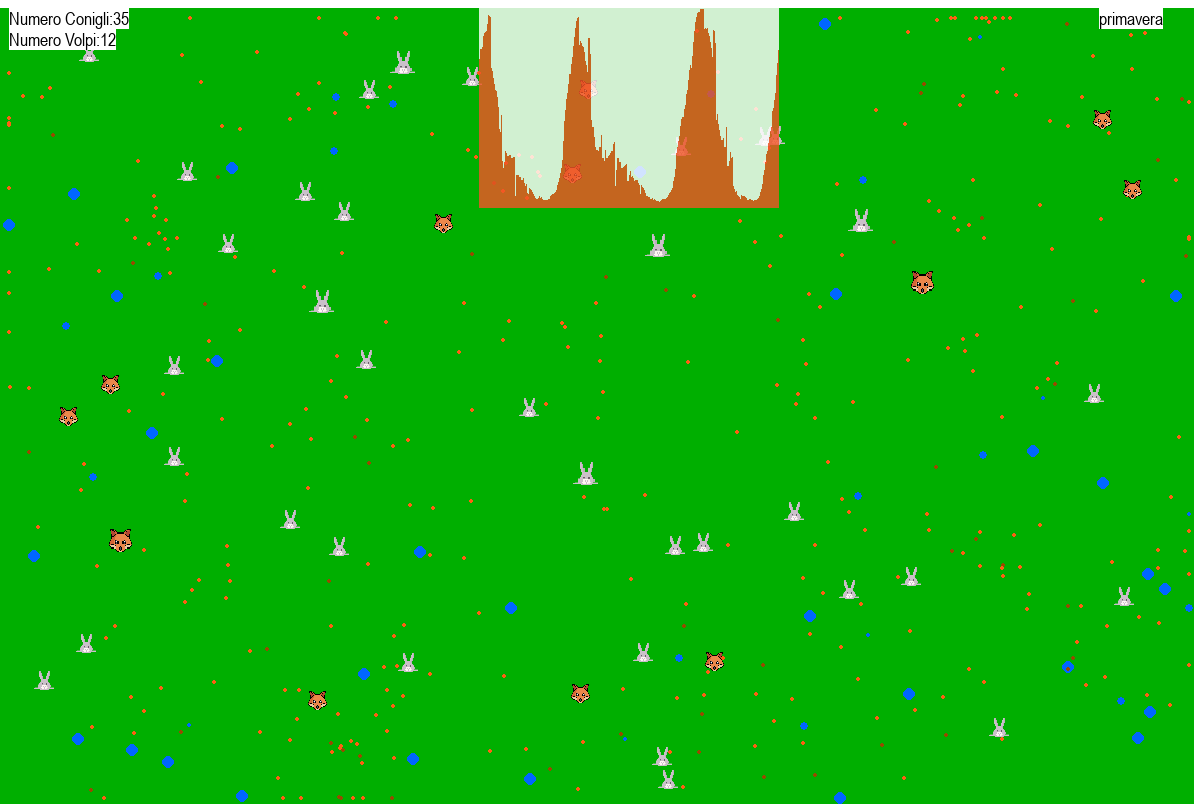
\includegraphics[scale = 0.50]{SIMULAZIONE.PNG}
\end{figure}




\newpage

\tableofcontents


\newpage

\section{Introduzione}
L'obiettivo del progetto è quello di realizzare una simulazione basata su agenti al fine di simulare il comportamento di un piccolo ecosistema naturale, costituito da una specie di predatori (volpi), una di prede (conigli), una vegetale (carote) e da alcuni specchi d'acqua (pozzanghere). Entrambe le specie animali presenti nell'ecosistema devono soddisfare alcuni bisogni fisiologici come il mangiare, il bere e il riprodursi. Per soddisfare la prima di queste necessità, le volpi si cibano dei conigli e i conigli a loro volta delle carote ed entrambi saziano la propria sete bevendo dalle pozzanghere che si formano nell'ambiente. Ogni singolo individuo è caratterizzato da alcune specifiche caratteristiche, quali soglia della fame, velocità di movimento, velocità di corsa, raggio di percezione, necessità di accoppiarsi e così via. Ogni individuo adulto è in grado di riprodursi e lo potrà fare solamente quando raggiunge il proprio periodo di fertilità ed incontra un altro individuo adulto della stessa specie. Ogni individuo che nasce in seguito all'accoppiamento erediterà i geni dai genitori ed inoltre il modello mette a disposizione la possibilità di simulare l'evoluzione genetica degli animali che popolano l'ambiente. 

Il fine del lavoro è quello di valutare come le varie configurazioni sviluppate si comportino rispetto ai modelli di riferimento presenti in letteratura. 



\section{Panoramica sugli ecosistemi naturali}
\subsection{Cos'è un ecosistema naturale}
Un ecosistema\cite{Vedantu} può essere definito come una comunità dove esseri viventi di specie differenti coesistono nello stesso ambiente fisico e interagisco vicendevolmente in modo da sviluppare un ciclo di vita e facilitare il flusso di energia e nutrienti.
Nello specifico, l'\textbf{european environment agency} definisce un ecosistema naturale come una particolare categoria di ecosistema dove l'impatto umano non ha avuto un' influenza maggiore di quello di qualsiasi altra specie autoctona e non ha influenzato la struttura dell'ecosistema dalla rivoluzione industriale. L'impatto umano esclude cambiamenti di proporzioni globali, come il cambiamento climatico dovuto al riscaldamento globale \cite{EEA}.
Il termine ecosistema venne per la prima volta usato in una pubblicazione dall'ecologista inglese \textbf{Arthur Tansley} nel 1935\cite{WikiEcosystem}.

Esistono due tipi di ecosistemi: quelli naturali e quelli artificiali. La prima categoria riguarda quelli che si sviluppano naturalmente e che possono svilupparsi e sopravvivere senza l'intervento umano. Ne sono esempi le foreste, le montagne, i fiumi, i prati e così via. Gli ecosistemi artificiali \cite{ArtificialEcosystems}, invece, hanno caratteristiche in comune con quelli naturali, ma sono creati e mantenuti dagli esseri umani. Essi sono più semplici rispetto a quelli naturali e sono quelli che più comunemente circondano l'esistenza umana. 

\subsubsection{La volpe rossa}
\label{volpe}
La volpe rossa (\emph{vulpes vulpes}) rappresenta il predatore scelto per la simulazione. Essa è la più grande delle volpi e il carnivoro più largamente diffuso, essendo presente in tutto l'emisfero boreale dal circolo polare artico all'Africa settentrionale, il nord America e l'Eurasia \cite{WikiVolpe}.
Questi animali possono misurare dai 75 ai 140 cm, per un peso che varia tra i 3 e gli 11 Kg. Il colore varia tra il giallo e il marrone e spesso è rossiccio. 

La volpe rossa vive generalmente in coppia con i cuccioli, ma talvolta è possibile osservare degli esemplari che vivono solitari oppure in gruppi di 4-6 adulti. Generalmente le volpi rosse cacciano in modo solitario e difendono il proprio territorio da sole durante l'estate e in coppia durante l'inverno. 

L'alimentazione della volpe rossa, nonostante sia classificato come animale carnivoro, comprende sia animali che vegetali. La dieta di questo animale è basata su una grande quantità di specie, dagli invertebrati ai piccoli mammiferi, uova rettili e piccoli anfibi. Tra i vegetali, la volpe rossa si ciba di vari tipi di frutti di bosco. In particolare, essa caccia i conigli appostandosi in modo furtivo e silenzioso per poi balzare tramite un rapido scatto sulla preda. 

Il periodo degli amori è molto variabile e cambia secondo la latitudine: in Italia ha luogo in inverno, tra dicembre e febbraio. I parti avvengono generalmente tra marzo e aprile. La femmina, dopo una gestazione di 7 settimane, partorisce in media da 3 a 5 piccoli, che vengono allattati per un mese. Le volpi si riproducono una sola volta all'anno. 

In natura, le volpi rosse possono raggiungere l'età di 12 anni.

\begin{figure}[h]
    \centering
    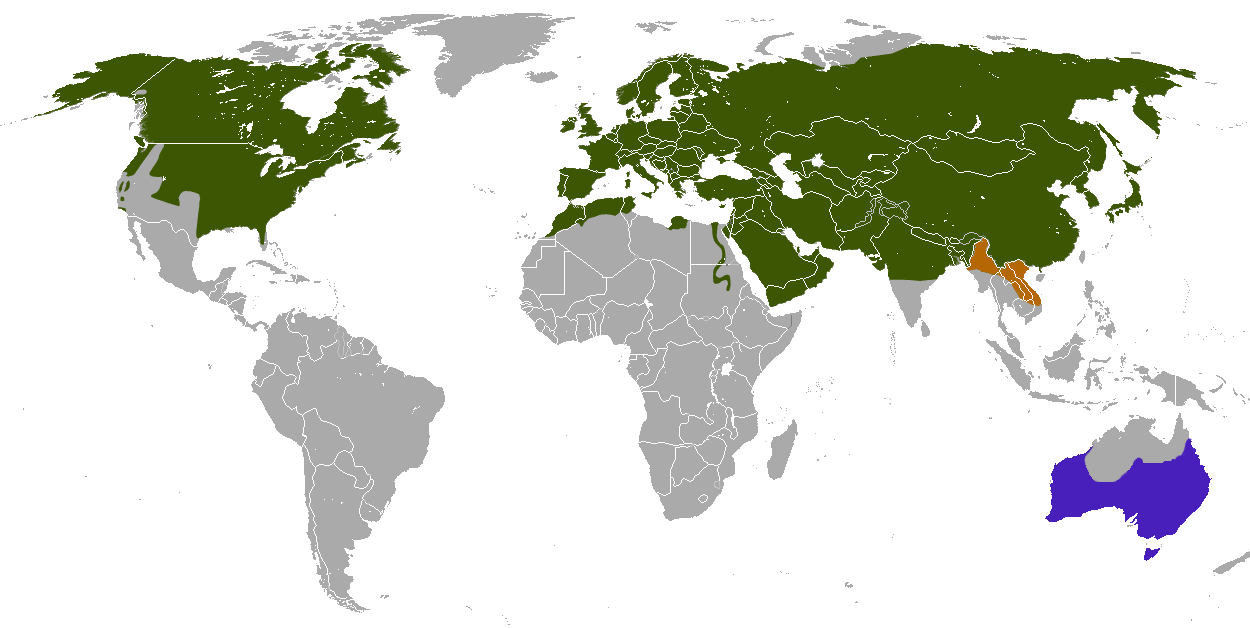
\includegraphics[scale = 0.3]{ArealeDellaVolpe.png}
    \caption{Areale della volpe. Le zone in verde indicano le aree dove la volpe è nativa, quelle blu dove è introdotta e quelle in arancione dove la presenza della volpe è dubbia. }
    \label{figArealeVolpe}
\end{figure}

Osservazioni sul campo\cite{RedFox} suggeriscono che le volpi siano miopi; possono attraversare la vegetazione senza incidenti, ma si avvicineranno agli oggetti fermi entro pochi metri a meno che un altro senso (come l'udito o l'olfatto) non le avvertano del pericolo o l'oggetto si muova. 

Le volpi hanno due orecchie altamente mobili, che possono essere mosse indipendentemente l'una dall'altra. Esse possono ruotare ciascun orecchio di circa 150 gradi in un'unica direzione, l'orecchio destro ruota in senso orario e l'orecchio sinistro in senso antiorario, per captare i suoni che provengono dai lati o dallo spazio retrostante. L'udito della volpe è molto sensibile ai suoni a bassa frequenza, come i fruscii emessi dalle prede. 

Per quanto concerne l'olfatto, la volpe rossa sfrutta questo senso non solo per identificare le prede, ma anche per comunicare con i propri simili e delimitare il proprio territorio.


\subsubsection{Il coniglio selvatico}
\label{coniglio}
Il coniglio selvatico europeo(\emph{Oryctolagus cuniculus}) rappresenta la preda scelta per la simulazione. Esso \cite{WikiConiglio} è un mammifero della famiglia dei leporidi, diffuso in gran parte dell'Europa (dal Portogallo alla Polonia, in Gran Bretagna e in alcune parti della Norvegia, Svezia e Ucraina), oltre al Nord Africa. Inoltre, i conigli selvatici sono stati introdotti in  Australia, Nuova Zelanda, Cile ed in numerose isole. 

\begin{figure}[h]
    \centering
    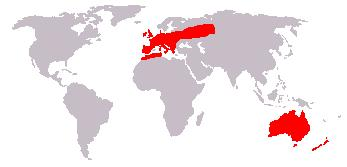
\includegraphics[scale = 1]{ArealeDelConiglioSelvatico.jpeg}
    \caption{Areale del coniglio selvatico.}
    \label{figArealeConiglio}
\end{figure}

Il coniglio selvatico predilige ambienti aperti, con clima secco e mite, ad altitudine non troppo elevata: il suolo dev'essere soffice o sabbioso, in modo da permettere all'animale di scavarsi la tana. Misura fino a 45 cm di lunghezza, per un peso che raggiunge i 2,5 kg: i maschi sono generalmente più grossi e robusti delle femmine. Si tratta di animali principalmente notturni e fortemente gregari, che possono vivere in colonie di grandezza direttamente proporzionale alla disponibilità di cibo. Una colonia tipo è composta da una decina di individui, senza distinzione di sesso. 

I conigli selvatici sono animali erbivori che si nutrono di diversi tipi di vegetali, dall'erba alle foglie e le carote.

I conigli sono famosi per la propria capacità riproduttiva: la femmina va infatti in estro ogni 21 giorni e tende a riprodursi durante i primi mesi dell'anno, anche se in condizioni favorevoli può allevare i piccoli durante tutto l'anno al ritmo di una cucciolata al mese. 

La gestazione dura un mese, al termine del quale vengono dati alla luce dai 3 ai 14 cuccioli. La femmina del coniglio può tornare a riprodursi appena dopo il parto\cite{Gattoni2019Apr}.  La speranza di vita di questi animali è di circa 9 anni, anche se in generale il 90\% degli esemplari muore prima di raggiungere l'anno d'età, a causa della forte pressione dei predatori. 

\subsection{La teoria della selezione naturale di Darwin}
Uno degli obiettivi del progetto è stato quello di simulare come l'evoluzione genetica e l'adattamento rispetto alle condizioni dell'ambiente influenzino la competizione tra le prede e i predatori. 

Il concetto di selezione naturale è stato introdotto per la prima volta dal biologo, naturalista e antropologo britannico \textbf{Charles Darwin} nel 1859 nella famosa opera \emph{L'origine delle specie}\cite{darwin1859}. Si tratta di un meccanismo alla base dell'evoluzione, secondo il quale il numero di individui che dimostrano di avere caratteristiche che si adattano in modo ottimale all'ambiente in cui vivono tende a aumentare in modo progressivo nel lungo periodo.
Gli individui di una specie si distinguono per alcune caratteristiche genetiche. La teoria della selezione naturale afferma che tale variabilità è causata da mutazioni genetiche casuali, ovvero non causate dall'adattamento degli individui all'ambiente. Con il passare del tempo, vengono selezionate (ovvero favorite) quelle mutazioni che permettono agli individui di adattarsi meglio all'ambiente in cui vivono. 

Gli individui che si adattano meglio a un certo habitat hanno la possibilità di procacciarsi più facilmente il cibo e si accoppieranno più facilmente rispetto agli altri individui della stessa specie che non presentano tali caratteristiche. I geni che fanno sì che l'individuo si adatti bene all'ambiente verranno trasmessi di generazione in generazione, mentre quelli inutili o dannosi vengono scartati. Questo porta all'evoluzione della specie che svilupperà caratteristiche che la rendono adatta a vivere e sopravvivere nell'ambiente. 

Uno dei più famosi esempi relativo alla selezione naturale è quello riguardante il collo delle giraffe. Nel corso di centinaia di migliaia di anni le mutazioni genetiche fecero in modo che alcuni individui di giraffe avessero un collo più lungo. Questa caratteristica si rivelò molto vantaggiosa perché permise a questi individui di raggiungere con agilità le foglie degli alberi più alti. In situazioni di scarsità di cibo questa caratteristica si rivelò determinante: gli individui con il collo lungo avevano maggiore probabilità di sopravvivere, di raggiungere l'età della riproduzione e di conseguenza di riprodursi e di trasmettere i propri geni (e di conseguenza anche la peculiarità del collo lungo) alle generazioni successive. 

I principi generali su cui si basa la teoria della selezione naturale, che verranno utilizzati per la creazione del modello utilizzato nella simulazione, sono i seguenti:
\begin{itemize}
    \item \textbf{Principio della variazione}: tra gli individui di una stessa popolazione esiste una variabilità di caratteri;
    \item \textbf{Principio dell'adattamento}: gli individui che meglio si adattano all'ambiente hanno dei caratteri che offrono un vantaggio in termini di sopravvivenza e di riproduzione;
    \item \textbf{Principio dell'ereditarietà}. Si tratta del principio secondo il quale le caratteristiche trasmissibili ai discendenti per mezzo della riproduzione sono localizzate all'interno dei geni degli individui. 
\end{itemize}

\section{Stato dell'arte}
\subsection{Sistemi complessi}
In letteratura esistono svariate definizioni, più o meno formali, di sistema complesso. In via del tutto generale, possiamo definire un sistema complesso come un sistema altamente strutturato, dinamicamente in evoluzione nel corso del tempo, il cui funzionamento è spesso complesso da spiegare o comprendere e in cui si verificano frequentemente interazioni multiple tra differenti componenti del sistema stesso. Alcune tipiche caratteristiche dei sistemi complessi sono le seguenti: 
\begin{itemize}
    \item Essi sono formati da elementi in continua interazione. Questi elementi prendono il nome di \textbf{agenti};
    \item La \textbf{non linearità}. Spesso emerge che nei sistemi complessi non esiste un rapporto lineare tra l'input e l'output.
    \item Possibilità di evolvere ed adattarsi nel tempo. 
    \item Robustezza e plasticità. 
\end{itemize}
Oltre ai sistemi complessi, possiamo definire altre due categorie di sistemi: i sistemi semplici e quelli complicati. La categoria dei sistemi semplici comprende quelli le cui relazioni causa-effetto sono ben note e documentate, oltre che prevedibili e ripetitive. Si può affermare che i sistemi semplici sono sistemi noti e conosciuti. Ne è un esempio la bicicletta. Un sistema complicato invece, è un sistema molto simile dal punto di vista delle relazioni causa-effetto rispetto ai sistemi semplici; la differenza risiede nel fatto che i sistemi complicati sono a più ampia scala e richiedono expertise specializzate. Sono sistemi che potremmo definire conoscibili e ne sono esempi le macchine, i razzi spaziali, i treni e così via. Infine, i sistemi complessi si differenziano dalle altre due categorie a causa del fatto che le relazioni causa-effetto possono essere apprese in retrospettiva, ma difficilmente risultano essere riproducibili o predicibili. Questa categoria è analizzabile seguendo l'approccio della simulazione. Ne sono esempi gli organismi viventi, il sistema nervoso umano e, ovviamente, gli ecosistemi naturali che sono oggetto del progetto descritto in questo documento. 
\subsection{Simulazione di sistemi complessi}
Come già affermato precedentemente, i sistemi complessi sono difficili da studiare e analizzare con un approccio teorico, è quindi opportuno utilizzare un approccio basato sulla simulazione. 

Gli scopi per cui si fa simulazione sono vari e possono essere riassunti nei seguenti punti:
\begin{itemize}
    \item Valutare piani e progetti operativi senza la necessità di metterli in atto nel mondo reale. Questo punto è molto importante perché attraverso la simulazione è possibile evitare di mettere in pratica un piano operativo per poi accorgersi che non può essere portato a termine in modo corretto. Questo permette di risparmiare risorse e fatica.
    \item Valutare teorie e modelli. Questo significa che la simulazione permette di comprendere meglio il sistema che stiamo studiando, valutandone le relazioni di causa-effetto che lo fanno evolvere in modo dinamico.
    \item Osservare un sistema che non è ancora stato realizzato nel mondo reale e che pertanto non è osservabile. Questa situazione si può verificare nel momento in cui il sistema è in via di sviluppo.
\end{itemize}

Come per tutti gli strumenti scientifici, anche per fare simulazione non esiste un unico approccio. Il primo approccio è quello macroscopico. Utilizzando questa tecnica, vengono specificati dei vincoli globali, rappresentati sotto forma di equazioni. Un esempio è il vincolo della conservazione della massa che impone che, qualunque cosa succeda nel sistema, la quantità di massa totale dovrà mantenersi costante nel tempo. Nei modelli macroscopici vengono stilate delle equazioni differenziali che indicano come variano le quantità aggregate nel corso del tempo. Si assume che gli individui siano tutti uguali e abbiano lo stesso comportamento e lo stesso atteggiamento. Lo svantaggio di questo approccio è che rende difficile catturare tutti gli aspetti della dinamica del gruppo di agenti che compongono il sistema. L'approccio macroscopico è particolarmente indicato per problemi di ottimizzazione in contesti specifici. Per esempio, questo metodo potrebbe rivelarsi utile per simulare l'evacuazione di un edificio e per verificare se tutte le persone all'interno di esso siano in grado di evacuare in meno di 10 minuti.
Uno degli esempi più famosi di modelli di simulazione macroscopici è il modello di Lotka-Volterra, descritto nella sezione \ref{sec:LV}. 

L'approccio alternativo prende il nome di simulazione basata sugli agenti o modellazione microscopica. Con questa metodologia l'unità analitica è costituita dal singolo individuo (che prende appunto il nome di agente) e non più dalle variabili aggregate come nell'approccio macroscopico. Il vantaggio sta nel fatto che i risultati dovrebbero evidenziare esattamente le stesse dinamiche descritte dai modelli macroscopici, oltre ad altre informazioni aggiuntive relative per esempio all'aspetto spaziale. Per esempio, nel contesto di un ecosistema naturale, alcuni modelli microscopici permettono di comprendere con un buon livello di confidenza dove si collocano i predatori e quali percorsi tendono a seguire. L'aspetto negativo riguarda il fatto che per realizzare un modello di questo tipo è necessario conoscere alcuni aspetti aggiuntivi del sistema e degli agenti che lo compongono. Per esempio, sempre prendendo in considerazione il modello dell'ecosistema naturale, è necessario conoscere come sono fatti i predatori, quali sono le loro caratteristiche, come cacciano, quali bisogni hanno e per le prede conoscere di cosa si cibano, come scappano o si nascondono dai predatori e così via. 

A prescindere dall'approccio che si usa, il ciclo di vita di un modello di simulazione è ben delineato. Infatti, per effettuare la corretta simulazione di un sistema complesso in generale si segue il ciclo di sviluppo riportato in figura \ref{figCicloSviluppo}.

Come si vede dall'immagine, le fasi dello sviluppo di una simulazione di un sistema complesso sono le seguenti: 
\begin{itemize}
    \item Definizione di un sistema target di riferimento, derivante dal processo interdisciplinare di analisi del fenomeno che si vuole studiare attraverso la simulazione.
    \item Operazione di modellazione e progettazione di un modello concettuale e di un simulatore del sistema in esame. 
    \item Esecuzione di simulazioni. Questo passaggio permette di acquisire una grande quantità di dati che risultano essere particolarmente utili nella fase successiva.
    \item Analisi dei risultati e validazione. In quest'ultima fase si sfruttano i dati raccolti dalle simulazioni effettuate e li si confrontano con i dati reali collezionati all'inizio del ciclo. Se i risultati della simulazione coincidono con le dinamiche osservate nel sistema reale (ovvero se il ciclo commuta), è possibile sfruttare il modello realizzato per fini esplicativi oppure predittivi; viceversa se dal modello sviluppato si ottengono dati che non coincidono con le osservazioni raccolte è necessario ripetere il ciclo e adattare il modello, sistemandone alcuni aspetti.
\end{itemize}

\begin{figure}
    \centering
    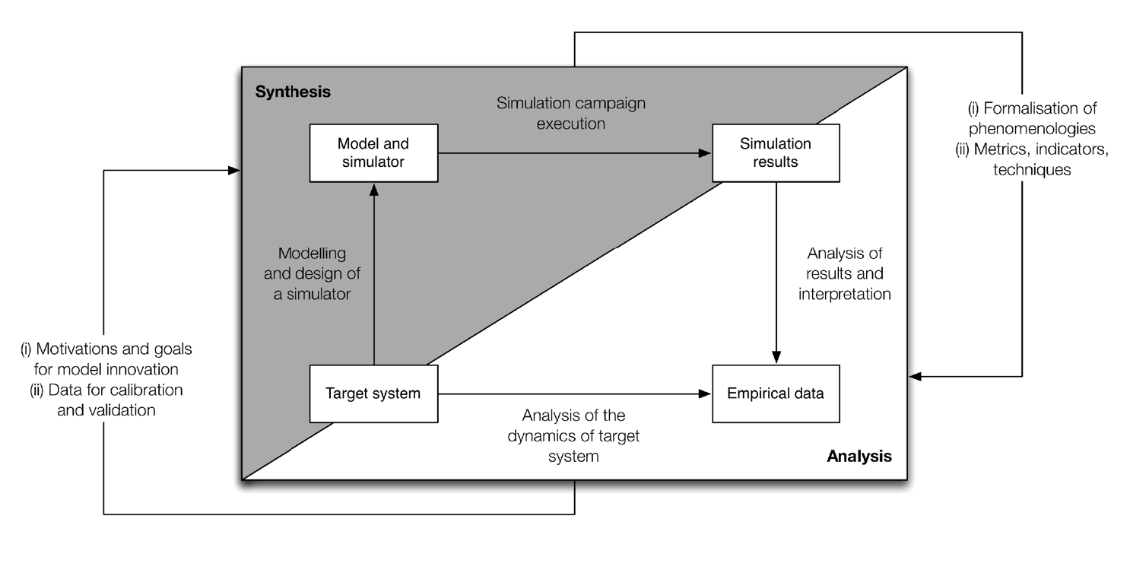
\includegraphics[scale = 0.6]{cicloSviluppoSimulazione.png}
    \caption{Schema che rappresenta il ciclo di sviluppo di una simulazione di un sistema complesso}
    \label{figCicloSviluppo}
\end{figure}

\subsection{Il modello Lotka-Volterra}
\label{sec:LV}
Il modello di Lotka-Volterra, noto anche come equazioni o modello preda-predatore, è il modello matematico più noto di analisi dei sistemi di tipo preda-predatore. Questo modello è stato proposto in modo indipendente dal matematico americano \textbf{Alfred J. Lotka} nel 1925 e dal fisico e matematico italiano \textbf{Vito Volterra} nel 1926. 

Il modello venne inizialmente proposto da \textbf{Alfred J. Lotka} nella teoria delle reazioni chimiche autocatalitiche pubblicata nel 1910 \cite{Goel}. Successivamente, dieci anni più tardi, Lotka estese il proprio modello, grazie anche al contributo del matematico sovietico \textbf{Andrey Kolmogorov}, a sistemi organici, utilizzando come esempio piante e specie di animali erbivori \cite{Lotka1920}. Infine, nel 1925 il matematico sfruttò il modello per analizzare l'interazione tra prede e predatori in un ambiente naturale\cite{Lotka1925}. L'anno successivo Vito Volterra si interessò allo stesso argomento poiché desiderava rispondere alla questione sollevata dal biologo \textbf{Umberto d'Ancona}\cite{Bacaer}. Egli aveva osservato che le percentuali di pesci cacciatori catturati dai pescatori erano aumentate durante la prima guerra mondiale. Questa osservazione lo stupì dato che durante gli anni di guerra la pesca venne praticata in misura molto minore rispetto agli anni precedenti. Volterra sviluppò il proprio modello in modo del tutto indipendente da Lotka e lo utilizzò per spiegare questo apparente paradosso. 

Il modello di Lotka-Volterra\cite{Artioli} descrive la dinamica di interazione fra due specie che convivono in uno stesso ambiente e sono in interazione tra di loro, definendo le seguenti ipotesi, che non sono necessariamente realizzabili in natura: 
\begin{enumerate}
    \item Le prede hanno sempre a disposizione una quantità illimitata di cibo. In altre parole, questo significa che le prede non potranno mai morire a causa della scarsità di cibo. 
    \item I predatori si cibano esclusivamente delle prede. 
    \item Il tasso di crescita delle popolazioni di entrambe le specie è proporzionale rispetto al numero di individui che compongono popolazioni stesse.
    \item L'ambiente, con il trascorrere del tempo, non evolve a favore di nessuna delle sue specie e i cambiamenti genetici sono irrilevanti. 
    \item La necessità di cibarsi dei predatori è limitata. 
\end{enumerate}

Sotto queste ipotesi, il modello di Lotka-Volterra prende la forma di un sistema di equazioni differenziali non lineari del primo ordine:
\[
\label{eqn:modelloGenerale}
\left\{
\begin{array}{cc}
\frac{dx}{dt}=\alpha x(t) - \beta x(t)y(t)\\
\frac{dx}{dt}=\delta x(t)y(t) - \gamma y(t)
\end{array}
\right.
\]

Dove: 
\begin{itemize}
    \item x(t) e y(t) rappresentano rispettivamente il numero di prede e predatori che popolano il sistema al tempo t.
    \item I parametri $\alpha$ e $\gamma$ indicano il tasso di crescita rispettivamente delle prede e dei predatori. In altre parole, indicano la differenza tra il tasso di nascita e il tasso di morte delle due specie.
    \item Il parametro negativo $-\beta$ indica come diminuiscono le prede in funzione dei predatori.
    \item Il parametro positivo $\delta$ indica come crescono i predatori in funzione delle prede. 
\end{itemize}

\noindent Nel caso specifico di un sistema che presenti solo prede, ricordando che esse hanno la possibilità di riprodursi senza limiti, l'unica cosa che può farne diminuire il numero sono i predatori.  
In questa situazione il sistema si può tradurre in un'unica equazione, che assume la seguente forma: 
\[
    \frac{dx}{dt} = \alpha x(t) 
\]
Anche in questo caso il parametro positivo $\alpha$ indica il tasso di crescita delle prede. 
La soluzione a tale equazione è 
\begin{equation}\label{eqn:soloPrede}
    x(t) = x(0)e^{\alpha t}
\end{equation}

\noindent Dove x(0) rappresenta il numero di prede presenti nel sistema al tempo 0.

\noindent Analizzando il grafico della funzione \eqref{eqn:soloPrede} riportato in \textbf{figura \ref{figPlotLotkaVolterraSoloPrede}}, è possibile notare che la funzione è monotona crescente. Questo implica che le prede tendono a crescere in numero, dato che l'unico fattore che ne potrebbe limitare la crescita è rappresentato dai predatori. 

\begin{figure}[h]
    \centering
    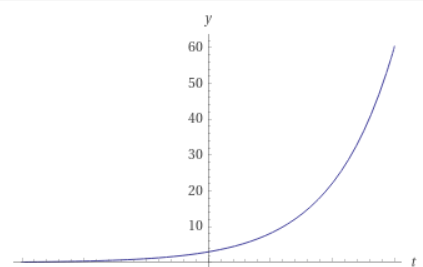
\includegraphics[scale = 1]{plotSoloPrede.PNG}
    \caption{Grafico della funzione \eqref{eqn:soloPrede} fissati i parametri x(0) e $\alpha$ rispettivamente a 3 e 2}
    \label{figPlotLotkaVolterraSoloPrede}
\end{figure}

\noindent Studiando invece, il caso specifico in cui il sistema sia abitato esclusivamente da predatori, il sistema di equazioni differenziali si riduce, anche in questo caso, ad una sola equazione che assume la seguente forma: 

\[
    \frac{dy}{dt} = -\gamma y(t) 
\]

Ancora una volta, il parametro negativo $-\gamma$ indica il tasso di morte dei predatori. 
Risolvendo l'equazione, otteniamo il seguente risultato:
\begin{equation}\label{eqn:soloPredatori}
    y(t) = y(0)e^{-\gamma t}
\end{equation}

\noindent Dove y(0) rappresenta il numero di predatori che popolano il sistema al tempo 0.

\noindent Analizzando il grafico della funzione \eqref{eqn:soloPredatori} riportato in \textbf{figura \ref{figPlotLotkaVolterraSoloPredatori}}, è possibile notare che la funzione è monotona decrescente. Questo implica che i predatori continueranno a diminuire in numero fino a estinguersi completamente. 

\begin{figure}[h]
    \centering
    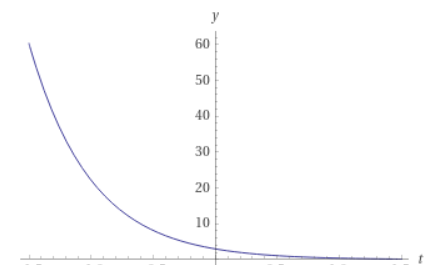
\includegraphics[scale = 1]{plotSoloPredatori.PNG}
    \caption{Grafico della funzione \eqref{eqn:soloPredatori} fissati i parametri y(0) e $\gamma$ rispettivamente a 3 e 2}
    \label{figPlotLotkaVolterraSoloPredatori}
\end{figure}

Il modello Lotka-Volterra generale, descritto dal sistema \ref{eqn:modelloGenerale} presenta il seguente andamento: 
\begin{itemize}
    \item Il numero di prede tende a crescere fintantoché il numero di predatori rimane basso;
    \item Al crescere delle prede, cresce anche il numero di predatori;
    \item Quando il numero di predatori è elevato e superiore rispetto a una certa soglia, il numero di prede tende a calare;
    \item Il diminuire delle prede viene accompagnato dalla contestuale diminuzione del numero di predatori;
    \item Nel momento in cui il numero di predatori è troppo basso, il numero di prede tende a risalire;
    \item tutto il ciclo si ripete;
\end{itemize}

Le soluzioni al sistema di equazioni non possiedono una espressione semplice in termini delle funzioni trigonometriche. Se si approssimano le soluzioni che si trovano in un intorno del punto di equilibrio stabile linearizzando il sistema, si ottiene un moto armonico semplice in cui la popolazione delle prede precede quella dei predatori con uno sfasamento di $\frac{\pi}{2}$, come visibile nella \textbf{figura \ref{fig:AndamentoLotkaVolterra}}\cite{WikiLotkaVolterra}.

\begin{figure}[h]
    \centering
    \includegraphics[scale = 0.7]{risultatoLotkaVolterra.PNG}
    \caption{Andamento del sistema Lotka-Volterra}
    \label{fig:AndamentoLotkaVolterra}
\end{figure}


\subsection{Modelli di simulazione di un ecosistema naturale multi-agente presenti in letteratura}
In questa sezione viene presentata una panoramica di alcuni dei modelli di simulazione multi-agente di un ecosistema naturale presenti in letteratura.

Al termine delle loro descrizioni, vengono messi in evidenza i punti di carenza di questi modelli. L'obiettivo del progetto è quello di superarli e quindi realizzare un modello più realistico rispetto a quelli esaminati.

\subsubsection{Modello preda-predatore agent based di Physics of Risk}
Il primo modello di simulazione di un ecosistema naturale che verrà presentato è quello disponibile al seguente link \href{https://rf.mokslasplius.lt/agent-based-prey-predator-model/}{Physics of Risk}\footnote{\url{https://rf.mokslasplius.lt/agent-based-prey-predator-model/}}.

Si tratta di un semplice modello realizzato sotto forma di applet HTML. In questo sistema l'ambiente è modellato in modo discreto, ogni preda è rappresentata da una cella colorata di bianco e ogni predatore è rappresentato come una cella colorata di nero. Il movimento è gestito in modo tale che l'agente che si muove verso il limite sinistro dell'ambiente, una volta oltrepassato, si troverà nella parte destra dell'ambiente. In modo del tutto analogo viene gestito il movimento verso l'alto e verso il basso. Ad ogni istante di tempo viene prelevata una cella in modo casuale dalla griglia. Se essa risulta essere vuota, allora non succede nulla, viceversa se è occupata da un agente allora viene selezionata una cella scegliendola in modo casuale tra quelle adiacenti ad essa. Prendendo in considerazione le due celle selezionate, all'inizio di ogni istante temporale vengono applicate le seguenti regole\cite{PhysicsofRisk}:
\begin{itemize}
    \item Se una cella è occupata da un predatore e l'altra da una preda, allora la preda viene mangiata, dopodiché il predatore da alla luce un figlio con una certa probabilità. Nel caso in cui sia nato un nuovo predatore, esso viene posizionato nella cella dove era posizionata la preda prima di essere stata mangiata dal predatore.
    \item Se le due celle sono occupate da due prede oppure da due predatori, allora non accade nulla.
    \item Se una cella è occupata da una preda e l'altra è libera, allora la preda da vita ad un cucciolo con una certa probabilità che occuperà la cella libera. 
    \item Se una cella è vuota e l'altra è occupata da un predatore, esso muore con una certa probabilità. 
    \item Se dopo l'applicazione delle regole sopra descritte non cambia nulla e la configurazione rende possibile il movimento dell'agente, allora esso si muoverà verso una cella non occupata. 
\end{itemize}

Provando ad eseguire diverse simulazioni con questo modello, si è constatato che esso in linea di massima risulta essere instabile. Infatti una delle due popolazioni (molto più frequentemente le prede) si estingue. Nonostante questo la dinamica del modello sembra essere attendibile, considerando che l'evoluzione del sistema nel corso del tempo è simile a quella descritta dal modello Lotka-Volterra. 

\subsubsection{Modello preda-predatore realizzati in NetLogo}
NetLogo è un ambiente programmabile di modellazione multi-agente, usato da migliaia di studenti, professori e ricercatori in tutto il mondo \cite{Netlogo}. NetLogo presenta un insieme piuttosto ricco di semplici modelli relativi a svariate discipline. Uno di questi è il modello denominato \textbf{Wolf Sheep Predation}. Esso si pone l'obiettivo di esplorare la stabilità dell'ecosistema preda-predatore. Per stabilità si intende il fatto che il sistema tende ad evolvere con fluttuazioni in termini di numerosità delle popolazioni delle specie che lo compongono, senza però che una abbia il sopravvento sull'altra, causandone la completa estinzione. Il sistema si dice quindi instabile nel caso in cui una o entrambe le popolazioni tendano ad estinguersi dopo un certo periodo di tempo.

NetLogo propone due varianti dello stesso modello. La prima, più semplice, viene chiamata \textbf{sheep-wolves} e prevede la presenza di soli due tipi di agenti: i lupi (predatori) e le pecore (prede). La seconda versione, quella più completa, oltre ai lupi e alle pecore include anche l'erba, attraverso la quale le pecore si cibano per mantenere alto il proprio livello di energia. In entrambi i modelli, sia le prede che i predatori hanno un certo livello di energia. In ogni istante temporale quello dei lupi diminuisce di un valore prestabilito. Essi per sfamarsi devono predare le pecore, così facendo il loro livello di energia diventerà massimo. Ogni qualvolta il livello di energia di un lupo dovesse raggiungere il valore zero, allora esso muore. Ogni lupo e pecora si riproduce con una probabilità prefissata ad ogni istante di tempo. Nella versione semplificata del modello la quantità di erba presente nell'ambiente è infinita, questo significa che ogni pecora non perde mai energia e muore solo nel caso in cui sia cacciata da un lupo. Questo implica anche che non viene modellata la crescita dell'erba. Questa versione, come affermato dalla documentazione di NetLogo, pur producendo risultati interessanti è in via definitiva instabile. La versione più completa presenta le seguenti differenze: viene aggiunta la modellazione dell'erba, le pecore (così come i lupi) devono cibarsi per poter acquisire energia e nel caso in cui dovessero esaurirla morirebbero. Una volta che l'erba viene mangiata da una pecora, si rigenera dopo un certo periodo di tempo prefissato. 

\begin{figure}[h]
    \centering
    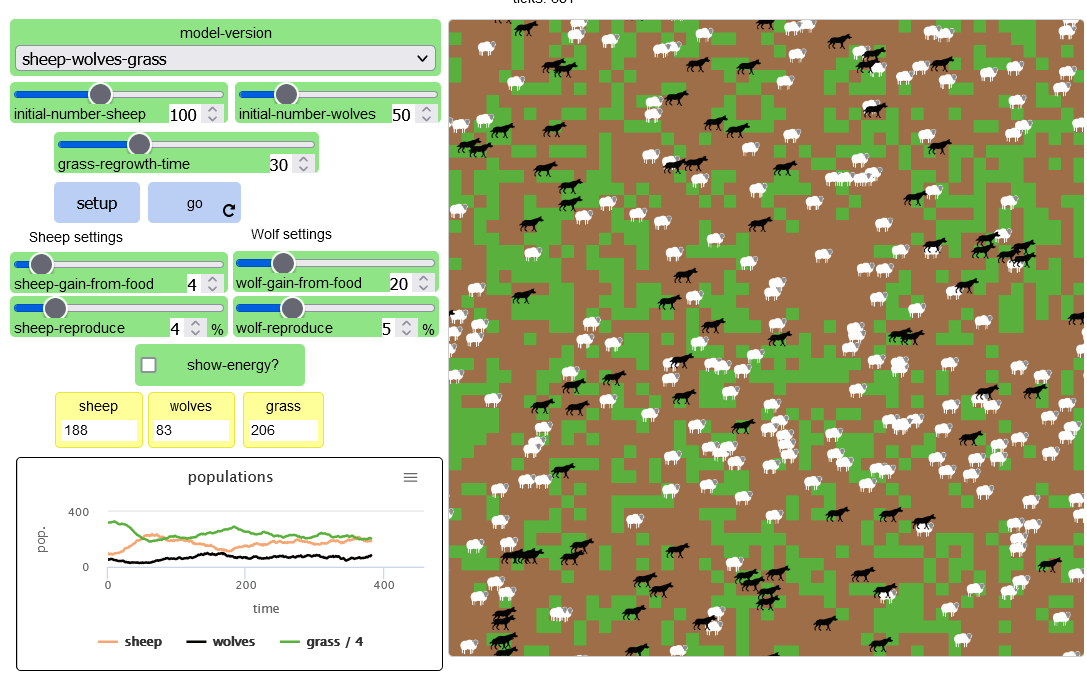
\includegraphics[scale = 0.5]{modelloNetLogo.png}
    \caption{La figura mostra il modello "Wolf Sheep predation" della libreria NetLogo}
    \label{fig:ModelloNetLogo}
\end{figure}

Oltre alle varianti appena descritte, in letteratura esistono svariati modelli multi-agente di simulazione di un ecosistema naturale realizzati in NetLogo. Gran parte di essi non si differenziano molto dai modelli standard della libreria di NetLogo. Di seguito, viene presentato quello proposto dai due ricercatori \textbf{Wilensky e Rand}\cite{WilenskyRand}, le cui principali caratteristiche sono le seguenti: 

\begin{itemize}
    \item \emph{Tipi di agenti}: pecore, lupi, erba;
    \item \emph{Proprietà degli agenti}: energia, posizione, direzione (solo per le pecore e i lupi), quantità (solo per l'erba);
    \item \emph{Comportamento degli agenti}: movimento, morte, riproduzione (solo per lupi e pecore), mangia-pecora (solo per i lupi), mangia-erba (solo per le pecore), ricrescita (solo per l'erba);
    \item \emph{Parametri}: Numero di pecore, numero di lupi, costo del movimento, energia acquisita dal cibarsi dell'erba, energia acquisita dal cibarsi delle pecore, tasso di ricrescita dell'erba.
    \item \emph{Andamento nel tempo}: Le pecore e i lupi si muovono $\rightarrow$ le pecore e i lupi muoiono $\rightarrow$ Le pecore e i lupi mangiano $\rightarrow$ Le pecore e i lupi si riproducono $\rightarrow$ l'erba ricresce
    \item \emph{Misure mostrate nei grafici}: Popolazione delle pecore in funzione del tempo, popolazione dei lupi in funzione del tempo e quantità di erba presente nel sistema sempre in funzione del tempo. 
\end{itemize}

Quest'ultimo modello appena descritto risulta essere stabile, ma, come descritto nella sezione successiva risulta essere troppo semplificato rispetto al contesto reale che intende simulare. 

\subsection{I limiti dei modelli presenti in letteratura}
I modelli descritti nella sezione precedente sono certamente validi, tuttavia risultano essere troppo semplificati rispetto al fenomeno reale che intendono simulare. 
In particolare, i limiti di questi modelli sono riassumibili nei seguenti punti:
\begin{itemize}
    \item Tutti i modelli presentati semplificano in modo estremo la modellazione dei fenomeni di accoppiamento e di riproduzione sia delle prede che dei predatori. Infatti, nessuno di essi simula il fenomeno naturale dell'accoppiamento degli individui. La riproduzione in tutti i casi è modellata in modo tale che ogni individuo in ogni istante di tempo abbia la possibilità di dare vita ad un cucciolo con una probabilità prefissata. Ovviamente, questa è una semplificazione estrema rispetto a ciò che accade nella realtà. Infatti in un contesto reale, come ampiamente descritto nelle sezioni \ref{coniglio} e \ref{volpe}, gli animali quando sentono la necessità di riprodursi, cercano un partner ideale col quale accoppiarsi. Solo dopo il processo di accoppiamento può avere luogo la riproduzione. 
    \item Una seconda importante limitazione di questi modelli riguarda il fatto che in natura ogni animale (che sia una volpe, una pecora o un lupo) non necessita solo di cibo per poter sopravvivere, ma ha bisogno anche di dissetarsi, bevendo quotidianamente una certa dose di acqua che può essere localizzata nell'ambiente in una pozzanghera, in un fiume, in un lago e così via.
    \item Tutti i modelli descritti non considerano il concetto di percezione degli animali. Come è noto e come descritto nelle sezioni precedenti, le volpi e i conigli in particolare, ma questo vale anche per i lupi e le pecore e più in generale per qualunque tipo di animale, hanno una certa percezione che deriva da quanto i suoi sensi (sopratutto udito, vista e olfatto) risultano essere acuti. Nessuno dei sistemi analizzati considera questo aspetto. Essi infatti sono stati sviluppati in modo tale che quando un predatore si trova sulla stessa cella di una preda, esso se ne ciba uccidendola. Anche questa è una semplificazione eccessiva della realtà: in natura i predatori spesso attuano delle strategie di caccia sfruttando i propri sensi. Questo significa che, in un contesto reale, i predatori non si muovono in modo casuale e quando si trovano esattamente a ridosso di una preda la cacciano, bensì tendono a seguire le tracce lasciate dalle prede e a inseguirle nel caso ne rilevino la loro presenza nelle vicinanze, grazie alla propria percezione. Vale lo stesso discorso per le prede; esse sfruttano i propri sensi per capire se c'è un pericolo nelle vicinanze e in caso affermativo tentano di fuggire, eventualmente cercando di nascondersi alla vista del predatore. 
    \item Un'ulteriore semplificazione della realtà adottata da questi modelli risiede nel fatto che le prede possono morire per due sole cause. Una preda infatti, può morire cacciata da un predatore oppure può morire di fame, a causa della scarsità di cibo presente nell'ambiente. Per quanto concerne i predatori invece, tutti e tre i modelli analizzati prevedono che essi possano morire solo a causa della scarsità di prede di cui cibarsi. Come facilmente immaginabile, in realtà queste non sono le uniche cause che possono portare alla morte in natura degli animali. Le prede e i predatori possono anche morire di sete, a causa della scarsità di acqua per esempio causata dal verificarsi di un lungo periodo di siccità, oppure possono morire di vecchiaia. 
    \item Ulteriore semplificazione adottata da questi modelli riguarda il fatto che in natura l'alternarsi delle quattro stagioni può portare ad effetti molto importanti nel contesto dell'ecosistema naturale simulato. La crescita dei vegetali non segue un andamento costante nel tempo. In primavera e in autunno, quando le piogge sono più frequenti, essi tenderanno a proliferare nell'ambiente, viceversa d'estate quando le piogge sono più rare, essi tenderanno a scarseggiare. Le stesse considerazioni valgono per le masse d'acqua. 
    \item Nessuno dei tre modelli considerati simula il passaggio dei geni dai genitori ai figli e la conseguente possibilità del verificarsi di un fenomeno evolutivo che può portare, col passare del tempo, allo svilupparsi di nuove caratteristiche nelle nuove generazioni di animali che gli permettono di adattarsi meglio all'ambiente in cui vivono.
\end{itemize}

\section{Obiettivo del progetto}
L'obiettivo del progetto è stato quello di realizzare un modello di simulazione multi-agente di un ecosistema naturale. Come illustrato nella sezione precedente, gran parte dei modelli di questo tipo presenti in letteratura sono piuttosto limitati, in quanto semplificano eccessivamente la realtà che intendono simulare. L'obiettivo quindi è stato quello di eliminare queste limitazioni. Dopo il processo di calibrazione dei parametri del modello si è optato per lo sviluppo di tre configurazioni dello stesso. La prima, la più semplice, ha portato a risultati non del tutto soddisfacenti, per questo motivo si è deciso di affinare il modello facendo sì che un certo numero di animali (sia prede che predatori) venissero reintrodotti nell'ambiente in modo periodico con una certa frequenza, così da simulare il fatto che altri individui entrano nell'ambiente, migrando dalle zone circostanti. I risultati ottenuti con questa seconda configurazione sono decisamente migliori e il modello è risultato essere notevolmente più realistico. Infine, si è deciso di estenderlo ulteriormente, introducendo la simulazione dell'evoluzione genetica degli animali che popolano l'ambiente. Il fine è stato quello di valutare tramite simulazione come l'evoluzione genetica permetta sia ai conigli che alle volpi di adattarsi alle condizioni ambientali. Per ciascuna delle tre varianti è stata eseguita un'analisi dei risultati e una comparazione con quelli relativi alle altre configurazioni. 

\section{Descrizione del modello}
Come già detto precedentemente, il modello sviluppato è un sistema multi-agente, composto da quattro agenti: i \emph{Conigli} (ovvero le prede), le \emph{Volpi} (ovvero i predatori), l'Acqua (ovvero le pozzanghere d'acqua attraverso le quali le prede e i predatori si dissetano) e le Carote (ovvero il vegetale con cui i conigli si sfamano). In questa sezione vengono illustrati l'ambiente, le quattro tipologie di agenti e i parametri del modello. Inoltre, per ognuno di essi, viene illustrato il valore finale scelto in seguito alla fase di tuning, con la quale si è cercato di rendere il modello stabile. 

\subsection{Ambiente}
L'ambiente è stato modellato nel seguente modo:
\begin{itemize}
    \item L'ambiente è \textbf{continuo}. Si è adottata questa scelta implementativa per rendere la simulazione più realistica. Infatti, l'unità di misura utilizzata per descrivere i movimenti e le percezioni degli agenti nello spazio è il singolo pixel, raggiungendo così un indice di granularità sufficientemente alto da considerare l'ambiente continuo.
    \item L'ambiente è \textbf{inaccessibile}. Questo significa che ogni agente non può, in ogni istante di tempo, ottenere informazioni complete, precise e aggiornate relative allo stato dell'ambiente stesso. Infatti ogni volpe è in grado di conoscere esclusivamente le informazioni che la sua percezione le permette di ottenere. Questo significa che una volpe può sapere se c'è un coniglio, uno specchio d'acqua oppure un'altra volpe con cui accoppiarsi nelle vicinanze, ma non può conoscere (e non è nemmeno necessario) il fatto che nella posizione diametralmente opposta alla sua si trova un altro individuo della sua specie, per esempio.
    \item L'ambiente è, inoltre, \textbf{dinamico}: nella finestra temporale nella quale ogni agente compie la decisione relativa al comportamento che deve tenere, l'ambiente può evolvere. In altre parole questo significa che esistono fattori esterni che influenzano e modificano l'ambiente mentre ogni agente valuta l'opportuna azione da effettuare. Per esempio, d'estate alcune delle pozze d'acqua vengono rimosse a causa del caldo e quindi l'ambiente evolve grazie ad un fattore esterno non gestibile dagli agenti.
    \item L'ambiente è \textbf{non deterministico}, ovvero ogni qualvolta un agente compie un'azione, non è possibile considerare come certo l'avvenimento dell'azione stessa. Infatti, alcune azioni sono state gestite tramite un processo regolato in modo stocastico e quindi non è certo che i loro effetti si realizzino effettivamente. Oltre a ciò, anche eventi esterni possono impedire la riuscita dell'azione che un agente ha prestabilito. Per esempio, se una volpe decide di predare un coniglio nelle vicinanze, non è garantito che possa riuscirci poiché possono intervenire svariati fattori esterni; per esempio il coniglio potrebbe nel frattempo morire di fame e quindi essere rimosso dall'ambiente prima che la volpe possa cibarsene. 
    \item Ulteriore caratteristica dell'ambiente è che esso risulta essere \textbf{episodico}. Episodico significa che ad ogni step temporale il comportamento di ogni agente è determinato considerando esclusivamente lo stato attuale del sistema. Gli agenti non sono dotati di memoria e non  mantengono traccia delle azioni precedenti. 
\end{itemize}

\subsubsection{Implementazione}
\label{sec:ambienteImplementazione}
\begin{figure}[h!]
     \centering
     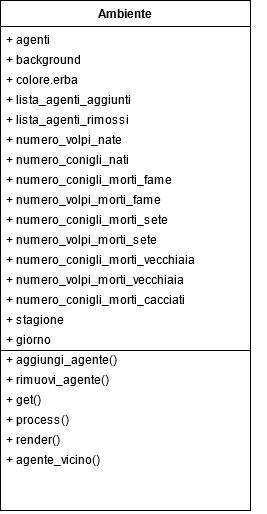
\includegraphics[scale = 0.7]{Ambiente.png}
     \caption{Diagramma della classe Ambiente}
     \label{fig:ambienteUML}
\end{figure}

L'ambiente è stato implementato attraverso un'apposita classe, le cui specifiche sono mostrate in figura \ref{fig:ambienteUML}. Gli attributi di questa classe includono: la lista di agenti presenti nell'ambiente, la lista di agenti rimossi dall'ambiente dopo la loro morte, la lista di agenti aggiunti in seguito alla loro nascita, una variabile di tipo stringa denominata \emph{stagione} che indica in quale stagione si trova attualmente la simulazione, una variabile di tipo floating point denominata \emph{giorno} che permette di tenere traccia del passare del tempo durante la simulazione, una variabile denominata \emph{background} utile in fase di render dell'ambiente, una tupla denominata \emph{colore\_erba} che permette di specificare il colore con cui l'ambiente deve essere colorato in ciascuna stagione e infine, una serie di variabili intere che permettono di raccogliere i dati della simulazione in corso.

L'ambiente può eseguire le seguenti operazioni: aggiungere un agente quando esso nasce, rimuovere un'agente quando muore, restituire l'oggetto che rappresenta uno specifico agente dato il suo identificativo, eseguire il render dell'ambiente, portare avanti la simulazione in ogni istante temporale (metodo process()) e ricercare l'agente che si trova più vicino ad un altro agente passato come parametro al metodo \emph{agente\_vicino}. 
Più nello specifico, il metodo \emph{process} si occupa di mettere in atto il comportamento di ogni agente in ciascun istante temporale, di aggiungere alla simulazione gli agenti contenuti nella lista denominata \emph{lista\_agenti\_aggiunti}, di rimuovere dalla simulazione gli agenti contenuti nella lista chiamata \emph{lista\_agenti\_rimossi} e infine, di rimuovere gli oggetti contenuti nelle due liste. Il metodo \emph{agente\_vicino} invece, viene richiamato dagli agenti di tipo Volpe o Coniglio nel momento in cui essi devono cercare una preda da cacciare oppure un compagno con cui accoppiarsi. Il metodo prende in input le coordinate attuali dell'agente, il raggio in cui cercare (ovvero la loro percezione) e il tipo di agente da cercare. Il metodo quindi restituisce l'oggetto che fa riferimento all'agente più vicino del tipo specificato se ne è presente uno nel raggio specificato, altrimenti non restituisce nulla.    
\paragraph{Parametri}

I parametri relativi all'ambiente sono i seguenti: 
\begin{itemize}
    \item \textbf{Dimensione dell'ambiente}. Questo parametro indica la dimensione in altezza e in lunghezza espressa in pixel della finestra nel quale viene eseguito il render grafico dell'ambiente. In seguito a diverse prove, si è constatato che la dimensione dell'ambiente in rapporto al numero di agenti che lo popolano non deve essere troppo elevata. Infatti se l'ambiente fosse troppo grande, allora gli agenti si disperderebbero al suo interno. D'altro canto è anche essenziale che la dimensione dell'ambiente non sia eccessivamente ridotta in proporzione al numero di agenti al suo interno e alla loro velocità di movimento. 
    \item \textbf{Probabilità pioggia} in primavera, estate, autunno e inverno. Questo parametro indica per ciascuna delle quattro stagioni con quale probabilità in ogni istante di tempo pioverà.
    \item \textbf{Quantità nuove pozzanghere} in primavera, estate, autunno e inverno. Indica, per ogni stagione in caso dovesse piovere in un istante temporale, quante pozzanghere verranno aggiunte all'ambiente. Rappresenta l'intensità del fenomeno atmosferico.
    \item \textbf{Probabilità aggiunta carote} in primavera, estate, autunno e inverno. Indica, per ogni stagione, la probabilità che in ogni istante di tempo venga aggiunta una carota in una posizione casuale nell'ambiente.
    \item \textbf{Numero iniziale di agenti}. Indica il numero di agenti di tipo Coniglio, di tipo Volpe, di tipo Acqua e di tipo Carota inseriti inizialmente nel sistema. 
    \item \textbf{Durata stagioni}. Indica la durata, espressa in istanti temporali, di ognuna delle quattro stagioni. 
    \item \textbf{Entità riduzione pozzanghere}. Questo parametro indica di quante unità in ogni istante temporale d'estate le pozzanghere vengono ridimensionate a causa del caldo che fa evaporare l'acqua. 
\end{itemize}
\vspace{2pt}
\paragraph{Tuning dei parametri}
\label{sec:tuningAmbiente}
Di seguito viene esposto il valore con cui sono stati settati i parametri descritti nel paragrafo precedente.
\vspace{13pt}
\begin{table}[h!]
\centering
{\renewcommand\arraystretch{1.6}
\begin{tabular}{l|cc}
 & \textbf{Larghezza (pixel)} & \textbf{Altezza (pixel)} \\ \hline
\textbf{Dimensione dell'ambiente} & 1200      & 800      
\end{tabular}}
\end{table}

\begin{table}[h!]
\centering
{\renewcommand\arraystretch{1.9}
\begin{tabular}{l|cccc}
& \textbf{Volpe} & \textbf{Coniglio} & \textbf{Acqua} & \textbf{Carota} \\ \hline
\textbf{Numero iniziale di agenti} & 25    & 75       & 200   & 250   
\end{tabular}}
\end{table}

\begin{table}[h!]
\centering
{\renewcommand\arraystretch{1.6}
\begin{tabular}{p{0.28\textwidth}|cccc}
& \multicolumn{4}{c}{\textbf{Stagione}} \\   
\hline
\textbf{Parametro} & \multicolumn{1}{l}{Primavera} & \multicolumn {1}{l}{Estate} & \multicolumn{1}{l}{Autunno} & \multicolumn{1}{l}{Inverno} \\
\hline
Probabilità pioggia  & 0.285\%  & 0.1\%  & 0.5\% & 0.4\% \\
Quantità nuove pozzanghere & rand(0,10) & rand(0,50) & rand(0,10) & rand(0,10) \\
Probabilità aggiunta carote & 33\% & 20\% & 10\% & 20\% \\
Durata stagioni & 500 & 500 & 500 & 500 \\
Entità riduzione pozzanghere & -  & 1  & - & -    
\end{tabular}}
\end{table}

\subsection{Agenti}
Il modello sviluppato è composto da un totale di quattro tipi di agenti: volpi, conigli, carote e pozzanghere d'acqua. Di seguito vengono descritte le caratteristiche generali i parametri e il comportamento di ognuno di essi. 

\subsubsection{Acqua}
Questo agente è il più semplice insieme all'agente \emph{Carota} e rappresenta gli specchi d'acqua (pozzanghere) attraverso i quali le volpi e i conigli hanno la possibilità di soddisfare il proprio bisogno di dissetarsi. Sono distribuite in modo casuale nell'ambiente e possono essere sfruttate dalle prede e dai predatori fino ad un massimo di tre volte prima di scomparire. Ne vengono aggiunte di nuove nell'ambiente con frequenza differente nelle quattro stagioni, come mostrato nella sezione \ref{sec:tuningAmbiente}.  

\subsubsection{Implementazione}
\begin{figure}[h!]
     \centering
     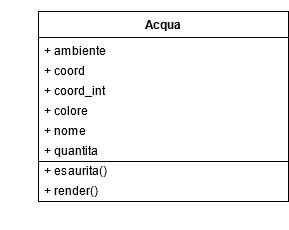
\includegraphics[scale = 0.7]{Acqua.png}
     \caption{Diagramma della classe Acqua}
     \label{fig:acquaUML}
\end{figure}

Gli attributi della classe Acqua sono i seguenti:
\begin{itemize}
    \item \textbf{ambiente}: è un riferimento all'oggetto Ambiente. 
    \item \textbf{coord}. Si tratta di un vettore in due dimensioni che rappresenta le coordinate dove si trova la rispettiva pozzanghera d'acqua nell'ambiente. 
    \item \textbf{coord\_int}. Analogo a coord, solo che \emph{coord\_int} è espresso tramite numeri interi e non decimali. 
    \item \textbf{colore}. Indica il colore con cui dovrà essere eseguito il render degli agenti di questo tipo.
    \item \textbf{nome}. Si tratta di una stringa con la quale vengono identificati gli agenti appartenenti a questa categoria. 
    \item \textbf{quantità}. Indica la dimensione della pozzanghera. Può assumere valori interi compresi tra 0 e 3. 3 significa che la pozzanghera può essere sfruttata ancora da 3 conigli e/o volpi prima di essere eliminata dall'ambiente, 0 significa che la pozzanghera deve essere rimossa, in quanto è stata già sfruttata 3 volte dalle volpi e dai conigli e quindi risulta essere esaurita. 
\end{itemize}

I metodi \emph{esaurita} e \emph{render} permettono rispettivamente di chiedere all'ambiente l'eliminazione dell'agente e di eseguire il render grafico degli agenti di questo tipo. 

\subsubsection{Carota}
Questa tipologia di agente rappresenta ciò di cui i conigli si cibano per potersi sostentare. Anche le carote, così come le pozzanghere d'acqua, sono inizialmente distribuite in modo casuale nell'ambiente. Le carote però, a differenza degli specchi d'acqua, una volta che sono state mangiate dai conigli scompaiono dall'ambiente e non possono essere ulteriormente mangiate da altri agenti. Così come per l'acqua, anche le carote vengono aggiunte sul territorio con frequenza che varia in base alla stagione, come illustrato nella sezione \ref{sec:tuningAmbiente}. 

\subsubsection{Implementazione}

\begin{figure}[h!]
     \centering
     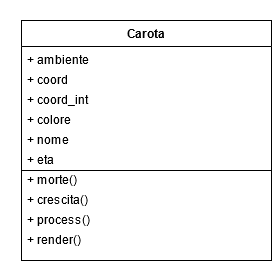
\includegraphics[scale = 0.7]{Carota.png}
     \caption{Diagramma della classe Carota}
     \label{fig:carotaUML}
\end{figure}
 Gli attributi degli agenti di tipo Carota sono i seguenti: 
\begin{itemize}
    \item \textbf{ambiente}. Si tratta di un riferimento all'oggetto della classe Ambiente. 
    \item \textbf{coord}. Si tratta di un vettore in due dimensioni, che rappresenta le coordinate che identificano la posizione della carota all'interno dell'ambiente. 
    \item \textbf{coord\_int}. Analogo a coord, la differenza risiede nel fatto che \emph{coord\_int} è espresso tramite numeri interi e non decimali. 
    \item \textbf{colore}. Indica il colore con cui dovrà essere eseguito il render degli agenti di questo tipo.
    \item \textbf{nome}. Si tratta di una stringa, utile per identificare gli agenti che appartengono a questa categoria. 
    \item \textbf{eta}. Indica da quanto tempo la carota è presente nell'ambiente. Una volta che la carota ha superato una soglia di vecchiaia verrà rimossa, in quanto marcita. 
\end{itemize}

I metodi della classe Carota sono i seguenti:
\begin{itemize}
    \item \textbf{morte}. Questo metodo viene invocato ogni qualvolta una carota viene mangiata da un coniglio, oppure marcisce. Esso chiede all'ambiente di rimuovere il rispettivo agente. 
    \item \textbf{crescita}. Questo metodo permette con una probabilità pari a 0.05\%, di far nascere una nuova carota nelle vicinanze dell'agente che lo richiama.
    \item \textbf{process}. Questo metodo, richiamato in ogni istante temporale della simulazione, esegue le seguenti operazioni: 
    \begin{itemize}
        \item richiama il metodo \emph{crescita}, descritto nel punto precedente;
        \item incrementa l'attributo \emph{eta} dell'agente di 0.03;
        \item nel caso in cui l'età della carota dovesse aver raggiunto un valore superiore a 2.5 cambia il colore con cui essa viene mostrata in modo da evidenziare che essa sta per marcire e quindi per sta per essere rimossa dalla simulazione;
        \item nel caso in cui la carota dovesse avere un'età superiore a 3, chiede all'ambiente di rimuovere l'agente. 
    \end{itemize}
    \item \textbf{render}. Questo metodo permette di eseguire il render grafico dell'agente nella corretta posizione dell'ambiente. 
\end{itemize}

\subsubsection{Coniglio e Volpe}
Gli agenti di tipo \emph{Coniglio} rappresentano le prede dell'ecosistema naturale che si intende simulare, mentre gli agenti di tipo \emph{Volpe} rappresentano i predatori. I due agenti sono stati implementati tramite le classi Coniglio e Volpe, che, come si può vedere dalla figura \ref{fig:ConiglioVolpeUML}, condividono la stessa struttura. 

\subsubsection{Implementazione}
\begin{figure}[h!]
     \centering
     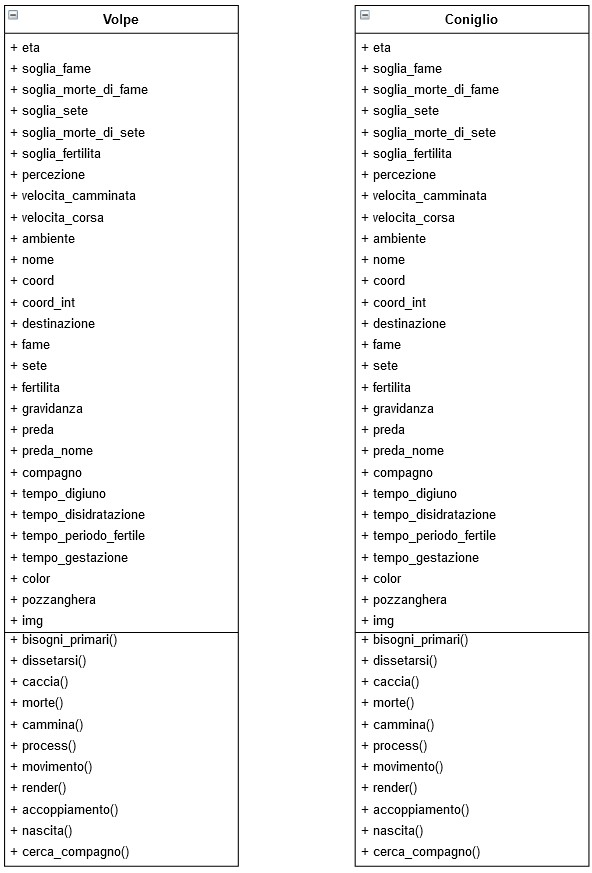
\includegraphics[scale = 0.7]{Animale.png}
     \caption{Diagrammi delle classi Coniglio e Volpe}
     \label{fig:ConiglioVolpeUML}
\end{figure}
Gli attributi relativi agli agenti Coniglio e Volpe sono i seguenti: 
\begin{itemize}
    \item \textbf{età}. Indica l'età dell'agente. In ogni istante temporale questo valore viene incrementato di 0.03. Conigli e Volpi di età superiore a 4 o inferiore a 0.5 hanno percezione e velocità di corsa dimezzata rispetto a quella degli animali adulti. Inoltre, Conigli e Volpi con età inferiore a 0.5 non possono accoppiarsi. 
    \item \textbf{percezione}. Questo attributo indica il raggio di percezione dell'agente. Un valore alto indica che l'agente può vedere e sentire predatori da grande distanza, viceversa un valore basso sta a significare che l'agente può vedere e percepire la presenza di altri agenti solo nel momento in cui si trovano a distanze ridotte rispetto al punto in cui esso si trova. 
    \item \textbf{ambiente}. Si tratta di un riferimento all'oggetto della classe Ambiente, precedentemente descritta. 
    \item \textbf{nome}. Si tratta di una stringa che indica il tipo di agente. 
    \item \textbf{coord}. Esso è un vettore in due dimensioni che identifica la posizione dell'agente in ogni istante temporale. 
    \item \textbf{coord\_int}. Indica la posizione attuale dell'agente tramite coordinate intere.
    \item \textbf{destinazione}. Indica la destinazione dell'agente. Inizialmente ogni coniglio e ogni volpe hanno una destinazione che viene fissata in modo casuale. Successivamente, nel momento in cui l'agente percepisce la necessità di accoppiarsi, cibarsi o dissetarsi e trova un agente che soddisfa il suo bisogno nelle vicinanze, questo parametro viene impostato in modo tale che la destinazione sia pari alle coordinate della posizione dell'altro agente. 
    Invece nel caso in cui l'agente non ha necessità allora la sua destinazione verrà impostata in modo casuale, in modo tale che esso si muova liberamente nell'ambiente. 
    \item \textbf{fame}. Si tratta di un valore booleano che indica se l'agente ha necessità di sfamarsi o meno. Inizialmente il valore è pari a False e nel momento in cui il numero di step temporali passati senza che abbia mangiato diventa superiore al parametro \emph{soglia\_fame} il suo valore viene impostato a True. 
    \item \textbf{sete}. Anche in questo caso si tratta di un valore booleano. Esso indica se l'agente necessita o meno di bere. Anche in questo caso, esso inizialmente è impostato a False e appena il tempo passato dall'agente senza bere diventa superiore al valore del parametro \emph{soglia\_disidratazione} il suo valore viene impostato a True. 
    \item \textbf{fertilità}. Si tratta di un valore booleano che indica se l'agente si trova in un periodo fertile o meno. 
    \item \textbf{gravidanza}. Anch'esso è un parametro di tipo booleano e indica se l'agente risulta essere in attesa di una cucciolata o meno. Nel primo caso, dopo un certo periodo di gestazione, esso darà alla luce i cuccioli. 
    \item \textbf{preda}. Fa riferimento ad un agente di tipo \emph{Carota} nel caso dei conigli e un agente di tipo \emph{Coniglio} nel caso delle volpi e rappresenta la preda identificata dall'agente per potersi cibare. 
    \item \textbf{preda\_nome}. Si tratta di una stringa che identifica il tipo di preda: coniglio per le volpi e carota per i conigli. 
    \item \textbf{compagno}. Esso rappresenta un agente con cui l'animale ha intenzione di accoppiarsi. 
    \item \textbf{tempo\_digiuno}. Si tratta di un parametro che indica il tempo passato dall'ultimo istante in cui l'agente si è cibato.
    \item \textbf{tempo\_disidratazione}. Indica quanti istanti temporali sono trascorsi dall'ultima volta che l'agente si è abbeverato in una pozzanghera. 
    \item \textbf{tempo\_periodo\_fertile}. Indica quanto tempo è passato dall'ultimo accoppiamento dell'animale. 
    \item \textbf{tempo\_gestazione}. Indica il tempo che deve passare dal momento in cui l'agente si è accoppiato prima che esso possa dare alla luce i cuccioli. 
    \item \textbf{pozzanghera}. Indica un agente di tipo Acqua che l'agente ha avvistato per potersi dissetare.
    \item \textbf{color}. Indica il colore con cui eseguire il render dell'agente. Questo attributo viene considerato solo nel momento in cui la simulazione viene lanciata con l'attributo GRAFICA impostato a False. Vedere la sezione \ref{sec:codice} per maggiori dettagli in tal senso. 
    \item \textbf{img}. Indica l'immagine con cui eseguire il render dell'agente. Questo attributo viene considerato solo per le simulazioni lanciate con l'attributo GRAFICA settato a True. Fare riferimento anche in questo caso alla sezione \ref{sec:codice} per maggiori dettagli. 
    \item \textbf{soglia\_fame}. Si tratta di una soglia superata la quale l'agente inizia ad avere necessità di cibarsi (di carote nel caso dei conigli e di conigli nel caso delle volpi).
    \item \textbf{soglia\_morte\_di\_fame}. Si tratta della soglia superata la quale l'agente morirà di fame. In altre parole, significa che se un coniglio o una volpe rimangono senza mangiare per un numero di istanti temporali superiore a tale soglia, allora esso morirà di fame.
    \item \textbf{soglia\_sete}. Indica la soglia oltre la quale l'agente inizia a percepire la necessita di dissetarsi. 
    \item \textbf{soglia\_morte\_di\_sete}. Così come per la fame, anche questa soglia è rappresentativa del fatto che se trascorre un numero di time step senza che l'agente abbia bevuto che è superiore rispetto a questa soglia, esso morirà di sete e verrà rimosso dall'ambiente. 
    \item \textbf{soglia\_fertilità}. Indica la soglia oltre la quale l'agente entra in un periodo di fertilità. Anche in questo caso, una volta passati un numero di time step senza che il coniglio si sia accoppiato, superiore a questa soglia, l'agente entra nel periodo di fertilità e quindi potrà cercare un compagno.
    \item \textbf{velocità\_camminata}. Questo parametro indica la velocità con cui si sposta l'agente in condizioni normali, ovvero quando non è inseguito da un predatore, non è alla ricerca di un compagno e non è alla ricerca di cibo con cui sfamarsi.  
    \item \textbf{velocità\_corsa}. Questo parametro invece, indica la velocità con cui l'agente si muove nelle seguenti condizioni: l'agente ha trovato un compagno con cui accoppiarsi, l'agente ha trovato una pozzanghera da cui abbeverarsi oppure l'animale ha trovato una preda di cui cibarsi nelle vicinanze.
    \item \textbf{eta\_morte\_vecchiaia}. Questo parametro indica a quale età le volpi e i conigli muoiono di vecchiaia.
\end{itemize}

\paragraph{Comportamento degli agenti Volpe e Coniglio}

Il metodo \emph{bisogni\_primari}, come si può intuire dal nome stesso, si occupa della gestione dei bisogni primari degli agenti di tipo Volpe e di tipo Coniglio. Entrambe queste categorie di agenti hanno tre necessità: cacciare (le volpi cacciano i conigli e i conigli si cibano delle carote) per non morire di fame, dissetarsi per non morire di sete e infine, accoppiarsi per potersi riprodurre. 

La gestione dei bisogni primari avviene come mostrato in figura \ref{fig:diagrammaComportamentale}. 
\begin{figure}
     \centering
     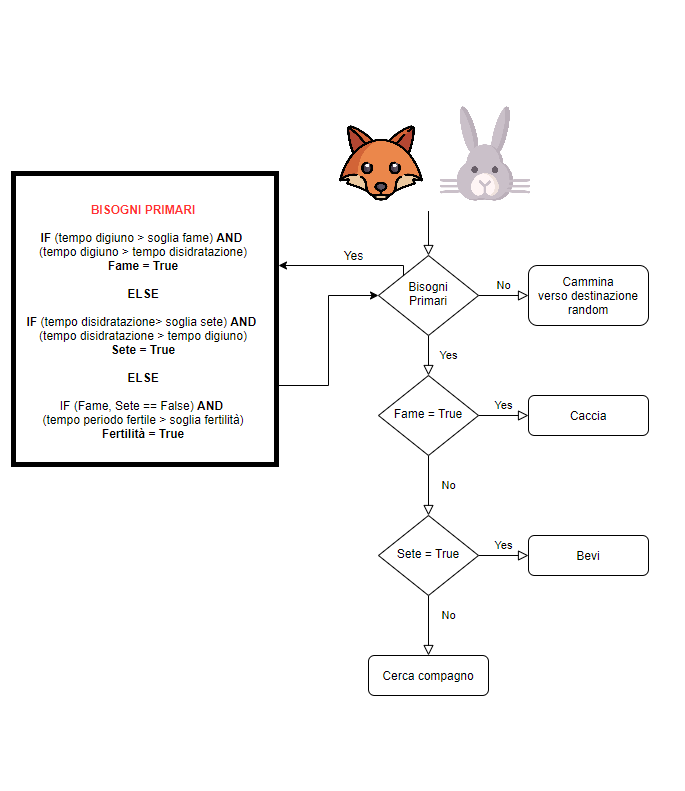
\includegraphics[scale = 0.75]{diagramma_comportamentale.png}
     \caption{Il diagramma in figura mostra il comportamento degli agenti di tipo Volpe e di tipo Coniglio ad ogni iterazione.}
     \label{fig:diagrammaComportamentale}
\end{figure}
Come si vede in tale immagine, per prima cosa si valuta se l'agente è morto di fame o di sete e nel caso viene richiamato il metodo \emph{morte} descritto in seguito. Successivamente si valuta se l'agente ha una delle tre necessità. Per far ciò, per prima cosa, viene considerato il tempo passato dall'ultima volta che l'animale si è cibato (valore memorizzato nella variabile \emph{tempo\_digiuno}) e il valore del tempo trascorso dall'ultimo istante in cui l'animale si è dissetato (memorizzato nella variabile \emph{tempo\_disidratazione}). Se il primo dei due valori è maggiore del valore di \emph{soglia\_fame} e del valore della variabile \emph{tempo\_disidratazione}, allora il valore della variabile booleana \emph{fame} viene settato a True. In seguito, si valuta se il tempo trascorso dall'ultima volta che l'animale si è dissetato è maggiore del valore di \emph{soglia\_sete} e del valore che indica il tempo trascorso dall'ultimo momento in cui l'animale si è sfamato. In caso affermativo, allora il valore della variabile booleana \emph{sete} viene settato a True. Infine, se il tempo trascorso dall'ultima volta che l'animale si è cibato è minore del valore \emph{soglia\_fame} e il tempo trascorso dall'ultima volta che l'animale si è dissetato è minore di \emph{soglia\_sete} e il tempo trascorso dall'ultima volta che l'animale si è accoppiato (memorizzato nella variabile \emph{tempo\_periodo\_fertile}) è maggiore del valore assunto dal parametro \emph{soglia\_fertilità}, allora il valore della variabile booleana \emph{fertilita} viene settato a True. 

In seguito a tali valutazioni, se nessuna delle tre variabili \emph{fame}, \emph{sete} e \emph{fertilita} ha assunto un valore pari a True, allora l'agente cammina verso una destinazione fissata in modo casuale all'interno dell'ambiente. Viceversa, se il valore della variabile \emph{fame} è diventato pari a True, allora l'agente inizia la procedura denominata \emph{Caccia}, descritta successivamente. Nel caso in cui la variabile \emph{fame} sia False e la variabile \emph{sete} sia True, allora l'agente inizia la procedura denominata \emph{Bevi}, descritta in seguito. Infine, nel caso in cui sia la variabile \emph{fame} che la variabile \emph{sete} sono pari a False e la variabile \emph{fertilita} ha assunto valore pari a True, allora l'agente inizia la procedura \emph{Cerca compagno}, descritta anch'essa successivamente in questa sezione. 

Il metodo \emph{caccia} permette di attivare la procedura denominata in modo analogo, attraverso la quale i Conigli possono cercare carote nelle vicinanze per potersi sfamare e le volpi possono cercare dei conigli nelle vicinanze in modo tale da poterli cacciare per poter soddisfare la propria necessità di cibarsi.
\begin{figure}
     \centering
     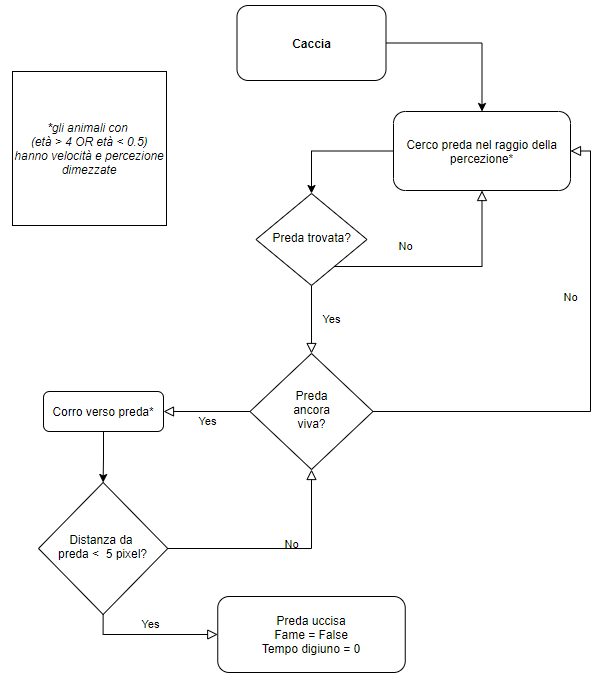
\includegraphics[scale = 0.75]{Caccia.png}
     \caption{Il diagramma in figura mostra come si comportano i conigli e le volpi quando hanno la necessità di cibarsi}
     \label{fig:diagrammaCaccia}
\end{figure}
Come visibile nella figura \ref{fig:diagrammaCaccia}, l'agente per prima cosa cerca se c'è una preda nell'area circolare avente come centro la posizione attuale dell'agente e come raggio la sua percezione. Se l'agente non trova una preda (una carota nel caso dei conigli, un coniglio nel caso delle volpi), allora esso camminerà verso un punto posizionato in modo casuale nell'ambiente e al prossimo istante temporale la procedura verrà ripetuta dall'inizio. 
Viceversa, nel caso in cui l'agente dovesse trovare una preda nei dintorni, allora l'ambiente comunica all'agente se la preda è ancora viva oppure no. Quest'ultima valutazione si rende utile per evitare il presentarsi di alcuni conflitti che occorrerebbero nel momento in cui un agente ha trovato una preda, ma prima che esso possa raggiungerla, un altro agente se ne ciba rendendola non più disponibile per il primo agente.
Nel caso in cui la preda non dovesse essere più presente nell'ambiente, allora l'agente si muove verso una destinazione random e ripete dall'inizio la procedura. Invece, nel caso in cui la preda dovesse essere ancora viva, l'agente inizia a correre verso di essa. Nel momento in cui la preda risulterà essere ad una distanza ridotta (inferiore a 5 pixel), allora la preda verrà uccisa, il parametro \emph{fame} dell'agente viene posto a False e l'attributo \emph{tempo\_digiuno} viene settato con un valore pari a zero. Se invece la distanza dovesse essere superiore a 5 pixel, l'agente chiede nuovamente all'ambiente se la preda è ancora viva e la procedura si ripete. 

Il metodo \emph{dissetarsi} permette di dare inizio alla procedura denominata \emph{bevi}, mostrata nel diagramma visualizzato nella figura \ref{fig:diagrammaBevi}. 
\begin{figure}
     \centering
     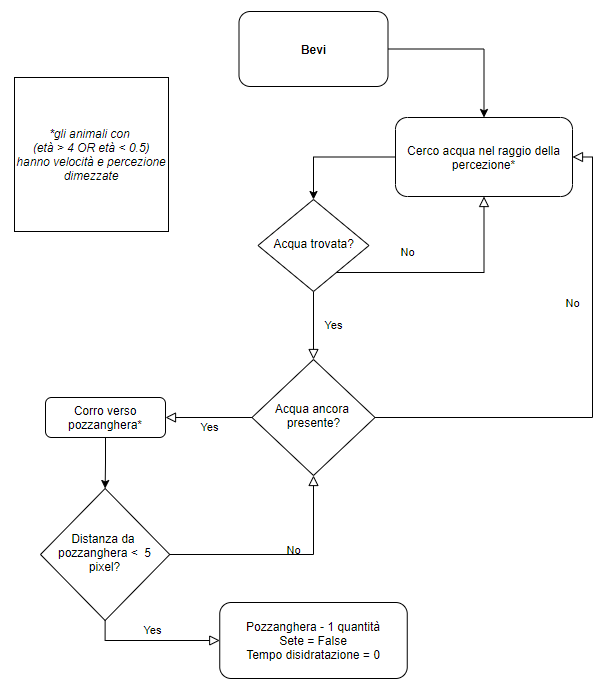
\includegraphics[scale = 0.75]{Sete.png}
     \caption{Il diagramma in figura mostra come si comportano i conigli e le volpi quando hanno la necessità di dissetarsi}
     \label{fig:diagrammaBevi}
\end{figure}
Questa procedura permette sia ai conigli che alle volpi di cercare una pozzanghera d'acqua per soddisfare la propria sete. Essa prevede in primo luogo che l'agente cerchi una pozzanghera nell'area circolare avente come centro la posizione attuale dell'agente e come raggio la percezione dell'agente stesso. Se l'ambiente comunica all'agente che non esiste una pozzanghera nei dintorni, allora l'agente si muove con destinazione casuale nell'ambiente e dal prossimo istante temporale la procedura viene riapplicata dall'inizio. Viceversa, nel caso in cui l'ambiente comunica all'agente che esiste una pozzanghera nelle vicinanze, allora esso inizia a correre verso la posizione della pozzanghera. In ogni istante temporale l'ambiente comunica all'agente se la pozzanghera è ancora presente nell'ambiente o meno (potrebbe accadere che altri agenti nel frattempo si sono diretti verso la stessa direzione e abbiano esaurito la pozzanghera). In caso negativo l'agente si dirige camminando verso una destinazione casuale e nel successivo istante temporale ripete la procedura dall'inizio. Se invece l'ambiente comunica all'agente che la pozzanghera non è stata esaurita da altri agenti, allora esso continua la corsa verso di essa. Questo ciclo si ripete fino a quando la distanza tra la pozzanghera e l'agente risulta inferiore a 5 pixel. In questa situazione l'agente si disseta, quindi il valore dell'attributo \emph{sete} diventa False, viene diminuita di una unità la dimensione della pozzanghera e l'attributo \emph{tempo\_disidratazione} dell'agente viene impostato con un valore pari a zero. 

Il metodo \emph{cerca\_compagno} permette di dare inizio alla procedura denominata in modo analogo, che permette alle volpi e ai conigli di cercare un animale della propria specie con cui accoppiarsi ed è illustrata con un diagramma visibile nella figura \ref{fig:diagrammaAccoppiamento}.
\begin{figure}
     \centering
     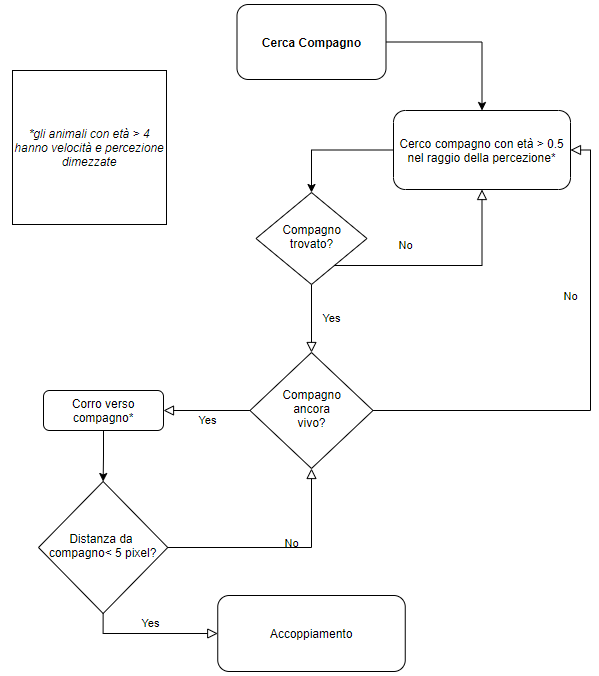
\includegraphics[scale = 0.75]{Cerca_Compagno.PNG}
     \caption{Il diagramma in figura mostra come si comportano i conigli e le volpi quando hanno la necessità di accoppiarsi}
     \label{fig:diagrammaAccoppiamento}
\end{figure}
Per prima cosa ogni agente che ha la necessità di accoppiarsi chiede all'ambiente se ci sono altri agenti dello stesso tipo e con età maggiore di 0.5 (i cuccioli non si possono accoppiare) nell'area circolare centrata nella posizione attuale dell'agente e di raggio pari alla percezione dello stesso.
In caso negativo l'agente si muove verso una direzione casuale nell'ambiente e dall'istante di tempo successivo riprende dall'inizio l'esecuzione della procedura. Viceversa in caso affermativo, l'ambiente comunica la posizione del candidato compagno più vicino. L'agente inizia a correre verso la posizione comunicatagli e in ogni istante temporale chiede all'ambiente se il compagno è ancora vivo. In caso negativo esso si sposta verso una destinazione casuale per poi ripetere l'intera procedura. Se invece l'ambiente comunica che il compagno è ancora vivo, allora l'agente continua la corsa verso di esso. Questa operazione viene continuamente ripetuta in ogni istante temporale fino a quando la distanza tra i due agenti risulta essere inferiore a 5 pixel. In questo caso l'accoppiamento vero e proprio può avere luogo, richiamando il metodo \emph{accoppiamento}. 

L'accoppiamento viene gestito in questo modo: gli attributi \emph{fertilita} dei due agenti coinvolti vengono impostati a False, gli attributi \emph{tempo\_periodo\_fertile}, che indicano quanto tempo è passato dall'ultimo accoppiamento dell'agente, vengono posti a 0 e inoltre l'attributo \emph{gravidanza} di uno dei due agenti viene impostato a True.
Dopo di questo, viene richiamato il metodo \emph{nascita} e dopo un periodo di gestazione, avviene la nascita  dei cuccioli(vedere il paragrafo \ref{sec:tuningAmbiente} per informazioni relative al numero di cuccioli che nascono ad ogni parto e ai tempi di gestazione delle due tipologie di agenti).

\vspace{20pt}

\noindent Nelle versioni del modello che non prevedono la gestione dell'evoluzione genetica i parametri \emph{soglia\_fame}, \emph{soglia\_morte\_di\_fame}, \emph{soglia\_sete}, \emph{soglia\_morte\_di\_sete}, \emph{soglia\_fertilità}, \emph{percezione}, \emph{velocita\_camminata} e \emph{velocita\_corsa} dei cuccioli vengono impostati seguendo il seguente principio: 
\[
    y = rand(min(x_1, x_2), max(x_1, x_2))
\]
Dove $y$ è il valore ereditato dal cucciolo e $x_1$ e $x_2$ sono i rispettivi parametri dei due genitori.  

Viceversa, nella versione del modello in cui è stata implementata l'evoluzione genetica,
ogni qualvolta nasce un cucciolo i parametri \emph{soglia\_fame}, \emph{soglia\_morte\_di\_fame}, \emph{soglia\_sete}, \emph{soglia\_morte\_di\_sete}, \emph{soglia\_fertilità}, \emph{percezione}, \emph{velocita\_camminata} e \emph{velocita\_corsa} dei cuccioli vengono ereditati dai genitori seguendo questo approccio:
\[
    y = rand(min(x_1, x_2), max(x_1, x_2)) + rand(-y1, y1) 
\]
Dove $y$ è il parametro ereditato dal cucciolo e $x_1, x_2$ sono i rispettivi parametri dei due genitori. Invece, $y_1$ è un offset appositamente scelto per ognuno degli otto parametri. Un valore grande implica che i cambiamenti genetici, anche nel breve periodo, siano più ampi, mentre se viene scelto un valore basso i cambiamenti genetici, almeno nel breve periodo,  risultano essere piuttosto contenuti. 
Un esempio di questo comportamento è mostrato in figura \ref{fig:EsempioEvoluzione}. 
\begin{figure}[h!]
     \centering
     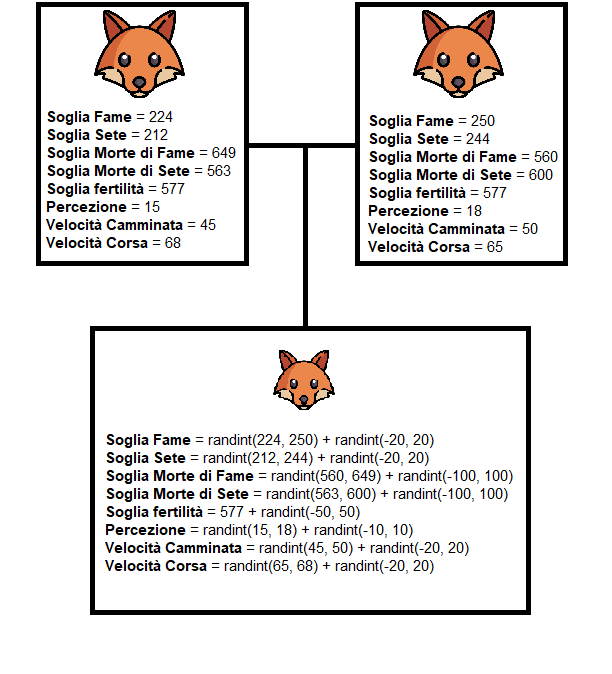
\includegraphics[scale = 0.8]{Accoppiamento_evoluzione.png}
     \caption{Il diagramma in figura mostra un esempio concreto di come viene gestita l'ereditarietà dei caratteri nel modello.}
     \label{fig:EsempioEvoluzione}
\end{figure}

\vspace{20pt}
\noindent Invece, il metodo \emph{morte} viene richiamato quando un animale muore di vecchiaia, muore di sete, muore di fame oppure muore cacciato da un predatore (ovviamente quest'ultimo caso è valevole solo per i conigli e non per le volpi). La prima situazione si verifica quando il valore \emph{eta} dell'agente supera il valore 4.5 nel caso dei conigli e il valore 5 nel caso delle volpi. Una volpe o un coniglio, invece muore di sete quando il valore \emph{tempo\_disidratazione} diventa maggiore del parametro \emph{soglia\_morte\_di\_sete}. Analogamente, un animale muore di fame quando il valore \emph{tempo\_digiuno} diventa superiore al parametro \emph{soglia\_morte\_di\_fame}. In tutti questi casi viene richiamato il metodo \emph{morte} che si occupa di aggiungere l'agente alla lista di agenti da rimuovere. Sarà poi compito dell'ambiente occuparsi della rimozione vera e propria dell'agente dall'ambiente. 

Il metodo \emph{cammina}, con l'ausilio del metodo \emph{movimento}, permette di spostare l'agente verso la propria destinazione con velocità pari a quella indicata nel parametro \emph{velocita\_camminata}. 

\newpage

Infine, il metodo \emph{process} si occupa del coordinamento di tutte le operazioni descritte fino ad ora. Esso viene richiamato in ciascun istante temporale e effettua le seguenti operazioni:
\begin{itemize}
    \item incrementare di una unità il valore delle variabili \emph{tempo\_digiuno} e \emph{tempo\_disidratazione};
    \item incrementare di 0.003 il valore dell'attributo \emph{eta} dell'agente;
    \item nel caso in cui l'età dell'agente sia maggiore di 0.5, aumentare il valore dell'attributo \emph{tempo\_periodo\_fertile} di una unità;
    \item valutare se l'agente ha raggiunto un'età tale per cui esso deve morire di vecchiaia e nel caso richiamare il metodo \emph{morte};
    \item richiamare il metodo \emph{bisogni\_primari} per la gestione delle necessità dell'agente;
    \item far muovere l'agente
\end{itemize}

In ultimo luogo, il metodo \emph{render} viene richiamato per eseguire il render grafico dell'agente all'interno dell'ambiente.

\vspace{1cm}

\paragraph{Tuning dei parametri}

\label{sec:tuningAnimali}
Nella tabella sottostante viene esposto il valore con cui sono stati settati i parametri descritti nel paragrafo precedente.

\vspace{1cm}

\begin{table}[hb]
\centering
{\renewcommand\arraystretch{1.6}
\begin{tabular}{l|cc}
\multicolumn{1}{c|}{\textbf{Parametro}} & \textbf{Volpe}   & \textbf{Coniglio} \\ \hline
soglia\_fame                   & rand(200; 250) & rand(200;250) \\
soglia\_morte\_di\_fame        & rand(550;650)  & rand(500;600) \\
soglia\_sete                   & rand(200;250)  & rand(200;250) \\
soglia\_morte\_di\_sete        & rand(550;650)  & rand(500;600) \\
soglia\_fertilita              & rand(500;600)  & rand(250;300) \\
percezione                     & rand(15;20)    & rand(15;20)   \\
velocita\_camminata            & rand(40;60)    & rand(40;60)   \\
velocita\_corsa                & rand(65;75)    & rand(65;75)   \\
eta\_morte\_vecchiaia          & 5              & 4.5
\end{tabular}}
\end{table}


\clearpage
\section{Ambiente di sviluppo e Codice}
\label{sec:codice}
Al fine di realizzare il progetto di simulazione, si è deciso di utilizzare il linguaggio di programmazione python, sfruttando la libreria pygame per realizzare l'interfaccia grafica. Pygame, come descritto nel sito ufficiale\cite{PyGame}, è un modulo python pensato per lo sviluppo di videogiochi che aggiunge funzionalità alla libreria multi-piattaforma SDL. Il suo utilizzo non è limitato esclusivamente allo sviluppo di videogame, ma è anche adatto per realizzare simulazioni multi-agente come nel caso del progetto corrente. Si è deciso di suddividere il codice in diversi moduli per garantirne una migliore chiarezza. Inoltre sono state usate diverse librerie aggiuntive, tra le quali:
\begin{itemize}
    \item \textit{\textbf{random}} per la gestione della simulazione è stato fatto un ampio utilizzo della generazione di valori pseudocasuali, attraverso questa libreria ed in particolare del metodo $randint(int_1, int_2)$, per ricreare al meglio la variabilità e l'entropia di un sistema complesso quale un ecosistema. Inoltre, si è deciso di  memorizzare dopo ogni esecuzione il \textbf{seed}, in modo tale da poter, in caso di necessità, lanciare una nuova esecuzione ottenendo esattamente i medesimi risultati.
    
    \item \textbf{\textit{pandas}} per la gestione dei dati attraverso l'utilizzo di dataframe e per la memorizzazione in file \textit{.csv} per effettuarne lo studio.
    
    \item \textbf{\textit{matplotlib}} per la creazione dei grafici, utili nella fase di analisi dei risultati.
    
    \item \textbf{\textit{\textit{os}}} e \textbf{\textit{sys}} per l'interfacciamento con il sistema operativo: gestione dell'evento di chiusura della finestra, creazione delle cartelle e memorizzazione dei file (grafici e .csv).
    
\end{itemize} 

Il codice, separato in vari moduli, è stato così suddiviso: \begin{itemize}
    \item \textbf{Simulazione}: è il modulo principale in cui si effettua la simulazione vera e propria. Qui sono implementati i vari agenti sotto forma di classi. Viene sfruttato il concetto dell'ereditarietà per rappresentare gli agenti Volpe e Coniglio, che ereditano alcuni parametri comuni dalla super-classe Animale. Viene inoltre gestita la raccolta dei dati, memorizzando delle “fotografie” dello stato della simulazione ad ogni 250 iterazioni, e tutto ciò che riguarda il "game loop", ovvero la logica con cui pygame gestisce le iterazioni. Anche il tempo di esecuzione è gestito in questo modulo e viene calcolato sulla base del lasso temporale che passa da un'iterazione e l'altra e serve per regolare la quantità di pixel che ogni agente percorre in movimento. Ad ogni 500 iterazioni un controllo va a gestire il cambio delle stagioni e ciò che ne comporta, come il cambio di render del terreno e di diversi parametri di gestione della pioggia e delle carote. Una volta chiusa la finestra di simulazione questo modulo salva i dati in un file \textit{.csv} che indirizzerà al modulo \textit{Plot}. Prima di ogni esecuzione è possibile regolare alcuni parametri, che servono per regolare il funzionamento e la visualizzazione della simulazione. Essi sono:
    \begin{itemize}
        \item \textbf{GRAFICA}: se settato a \textit{True} gli agenti animali verranno visualizzati con sprite 2D, se settato a \textit{False} gli agenti animali saranno visualizzati come dei semplici pixel colorati. Quest'ultima configurazione è particolarmente adeguata per garantire una migliore fluidità nell'esecuzione della simulazione, sopratutto nel momento in cui il numero di agenti da visualizzare a schermo risulta essere particolarmente elevato.
        \item \textbf{EVOLUZIONE:} se settato a \textit{True} verrà lanciata la simulazione nella configurazione con evoluzione. Questo implica, come descritto nel paragrafo precedente, che ogni qualvolta nasce un cucciolo, esso erediterà i caratteri dei genitori ed eventualmente verrà applicata una mutazione, in modo tale da studiare il meccanismo di selezione evolutiva dei geni. Viceversa, se settato a \textit{False} la simulazione verrà lanciata in modalità senza evoluzione. In questo caso il fenomeno della riproduzione degli animali porterà alla nascita di cuccioli i cui geni sono ereditati dai genitori senza che si presenti alcun tipo di mutazione. 
        \item \textbf{REINSERIMENTO:} se settato a \textit{True} la simulazione viene lanciata in modalità con reinserimento. Questo significa, come già descritto nei paragrafi precedenti, che ogni qualvolta si manifesta un cambio di stagione verranno inseriti nell'ambiente alcuni nuovi animali. Viceversa, se settato a \textit{False} non ci sarà alcun reinserimento.
        \item \textbf{NUMERO CONIGLI/VOLPI/POZZANGHERE/CAROTE:}  rappresenta il numero di agenti che all'inizio della simulazione popoleranno l'ambiente.
        \item \textbf{PROBABILITA\_CRESCITA\_CAROTE:}  rappresenta la probabilità che ad ogni iterazione una carota generi un'altra carota nelle vicinanze.
        \item \textbf{QUANTITA\_ACQUA:}  rappresenta la dimensione della pozzanghera, ovvero il numero di volte che essa può essere sfruttata da un animale prima che si esaurisca e quindi venga rimossa.
        \item \textbf{WIDTH/HEIGHT:}  rappresentano la dimensione della finestra di visualizzazione della simulazione, cambiarli non modifica solo l’aspetto visivo, ma va ad alterare anche l’esito della simulazione stessa a causa del fatto che vengono modificate le distanze tra gli agenti e questo può avere un impatto importante sull'esito della simulazione.
    \end{itemize}
    
    \begin{figure}[h!]
	\begin{subfigure}{\textwidth}
    \centering
     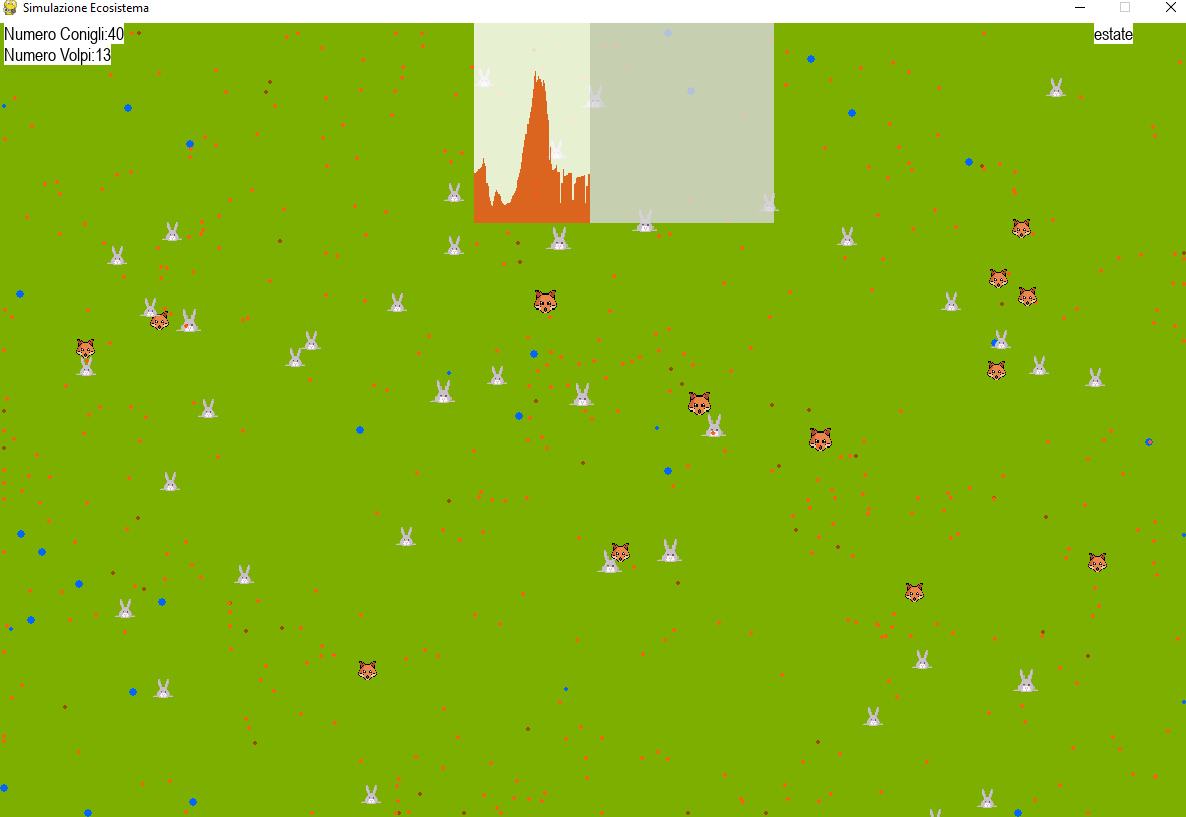
\includegraphics[scale = 0.3]{SIMULAZIONE-GRAFICA.PNG}
     \caption{GRAFICA = True}
     \label{fig:LVPhaseSpace}
	\end{subfigure}
	\begin{subfigure}{\textwidth}
		\centering
     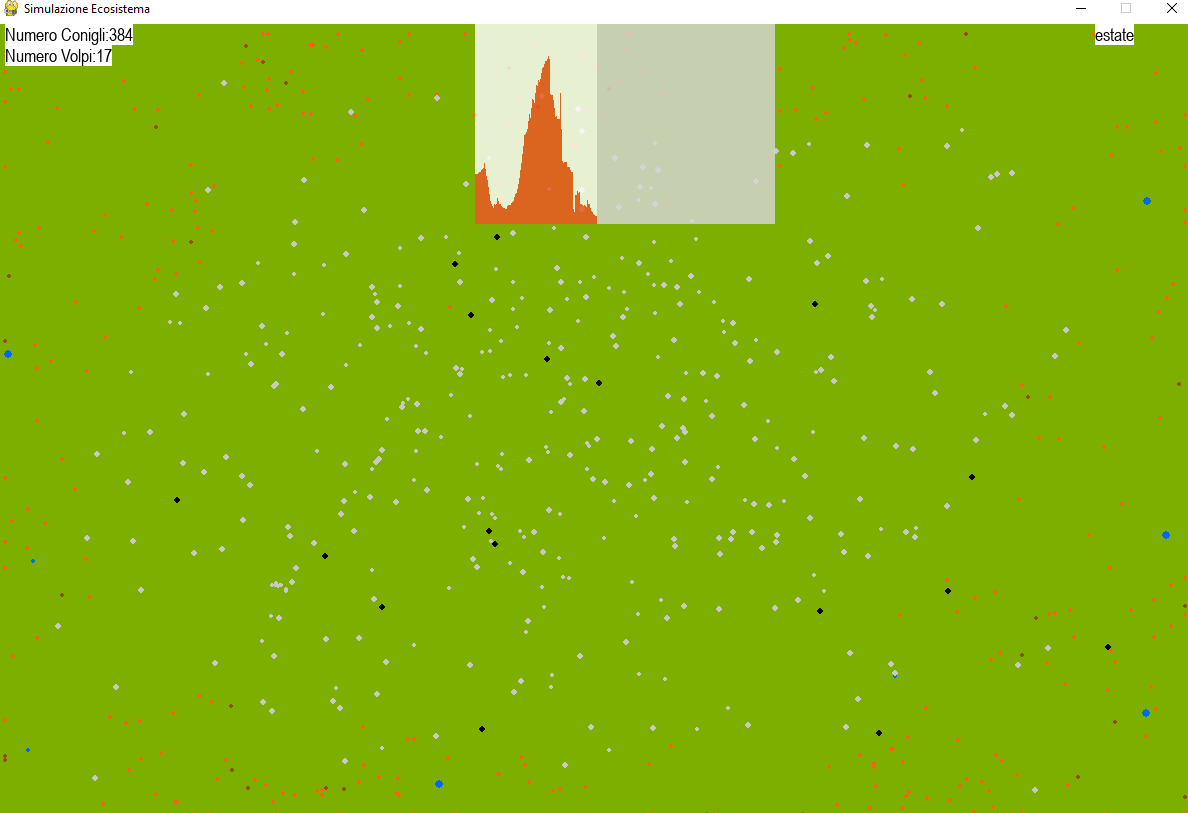
\includegraphics[scale = 0.3]{SIMULAZIONE-NOGRAFICA.PNG}
     \caption{GRAFICA = False}
     \label{fig:conigliVolpi}
	\end{subfigure}
	\caption{Visualizzazione della simulazione}
\end{figure}
    
    \item \textbf{Ambiente:} modulo inizializzato all'interno di \textit{Simulazione} che gestisce e regola l'ambiente della stessa. Al suo interno sono dichiarati i metodi per aggiungere, rimuovere, processare ed effettuare il render degli agenti. Inoltre vi sono inizializzate alcune variabili, descritte nel paragrafo \ref{sec:ambienteImplementazione}.  

\begin{figure}[h!]
	\hspace{-5mm}
	\begin{subfigure}{.5\textwidth}
         \centering
         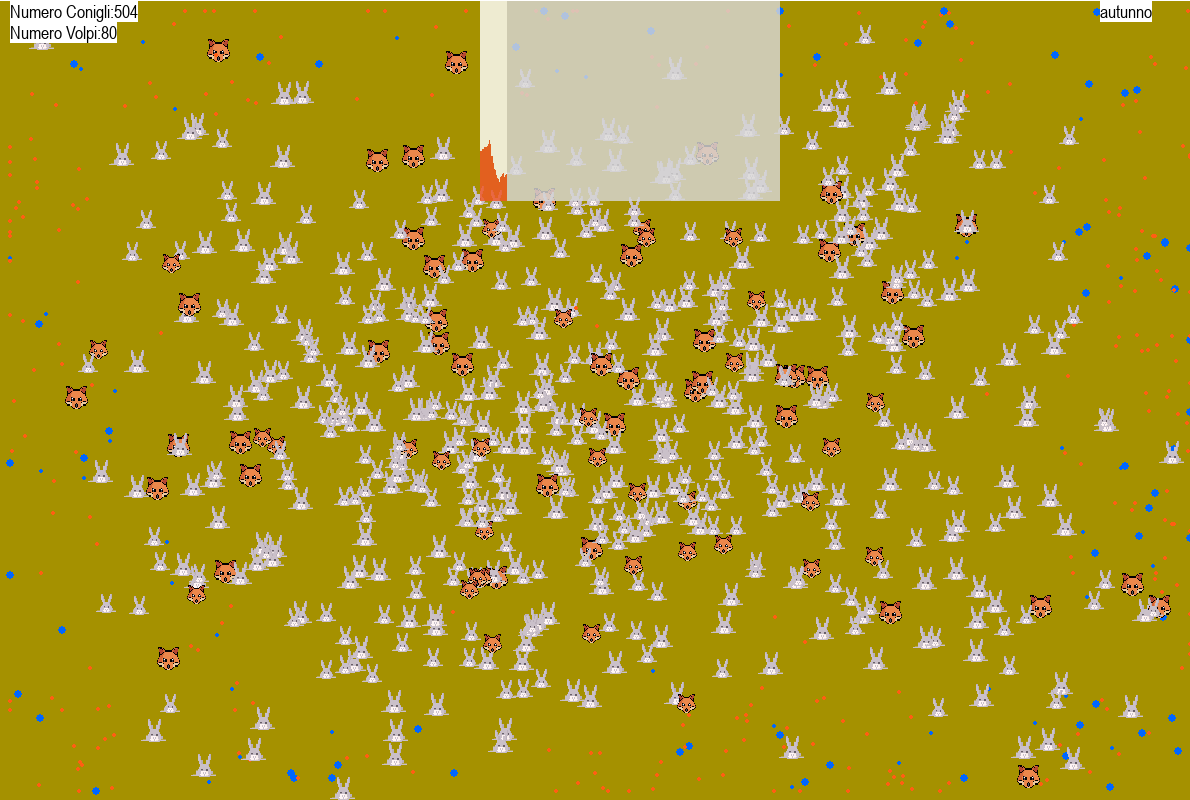
\includegraphics[scale = 0.2]{SIMULAZIONE_Autunno.PNG}
         \caption{Autunno}
         \label{fig:autunno}
	\end{subfigure}
	\begin{subfigure}{.5\textwidth}
		\hspace{7mm}
		\centering
        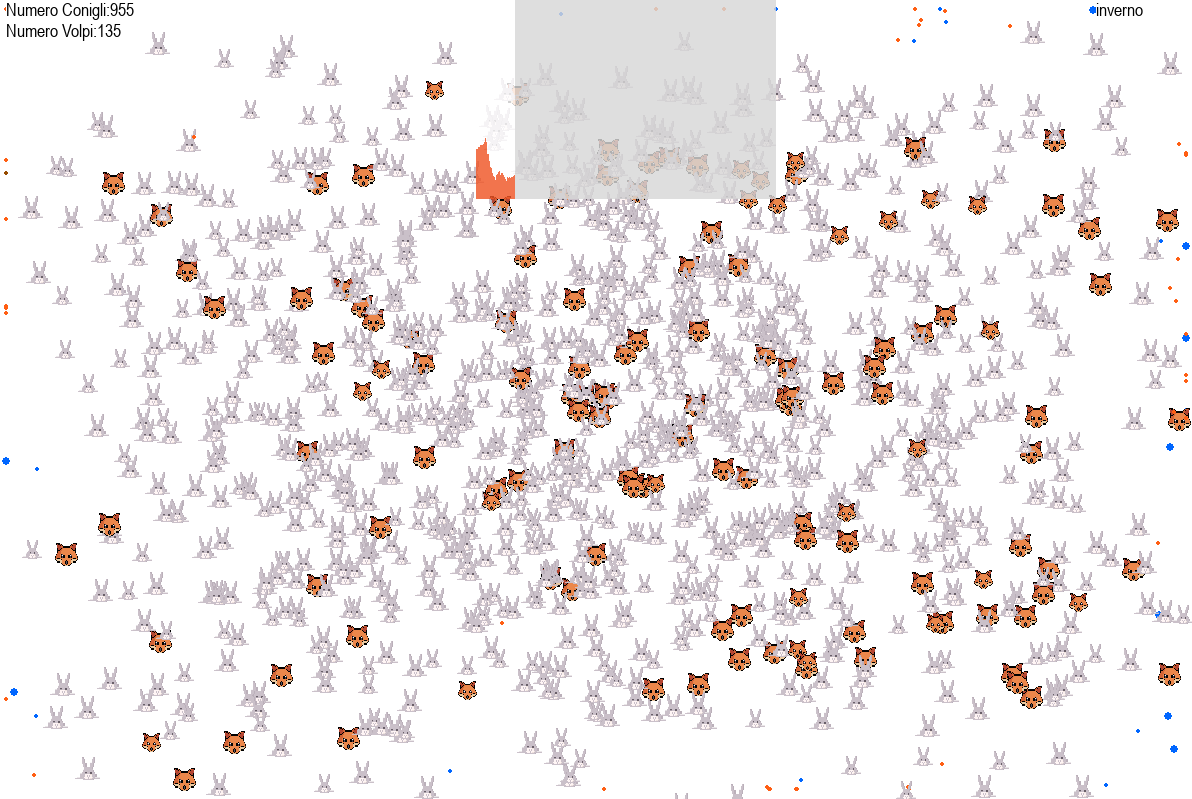
\includegraphics[scale = 0.2]{SIMULAZIONE_Inverno.PNG}
        \caption{Inverno}
        \label{fig:inverno}
	\end{subfigure}

	\hspace{-5mm}
	\begin{subfigure}{.5\textwidth}
         \centering
         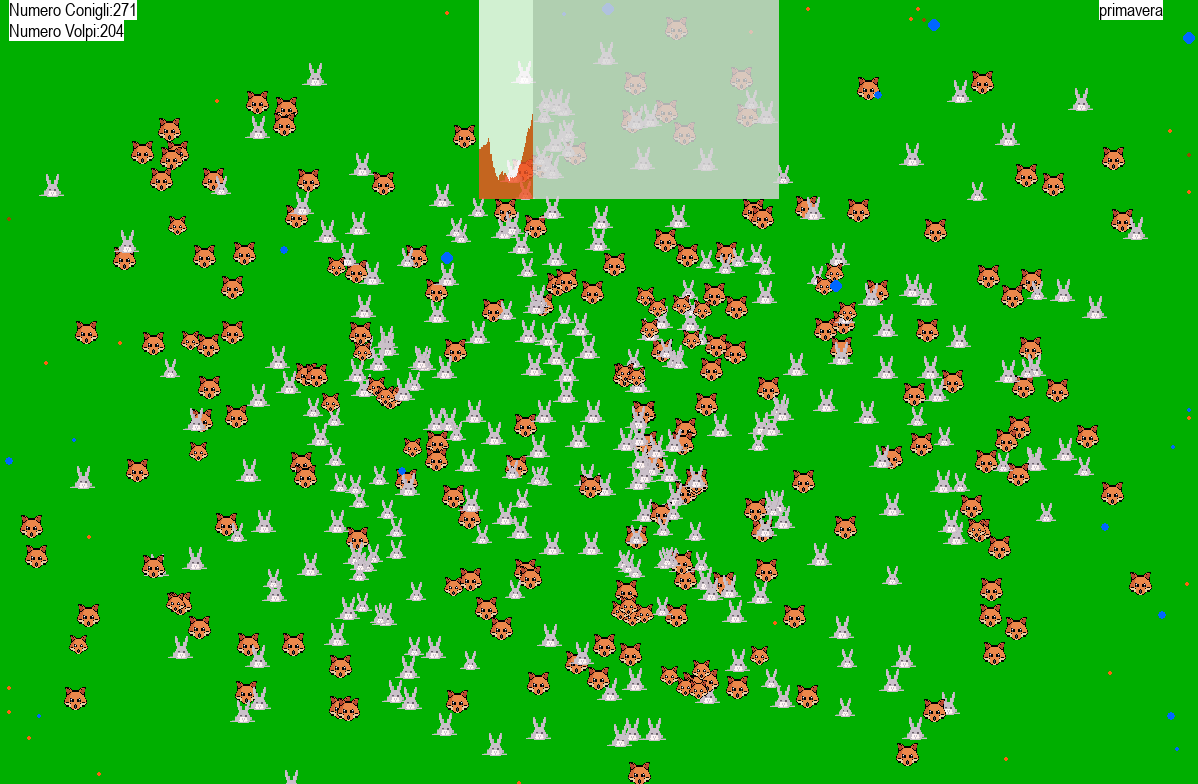
\includegraphics[scale = 0.2]{SIMULAZIONE_Primavera.PNG}
         \caption{Primavera}
         \label{fig:primavera}
	\end{subfigure}
	\begin{subfigure}{.5\textwidth}
		\hspace{7mm}
		\centering
        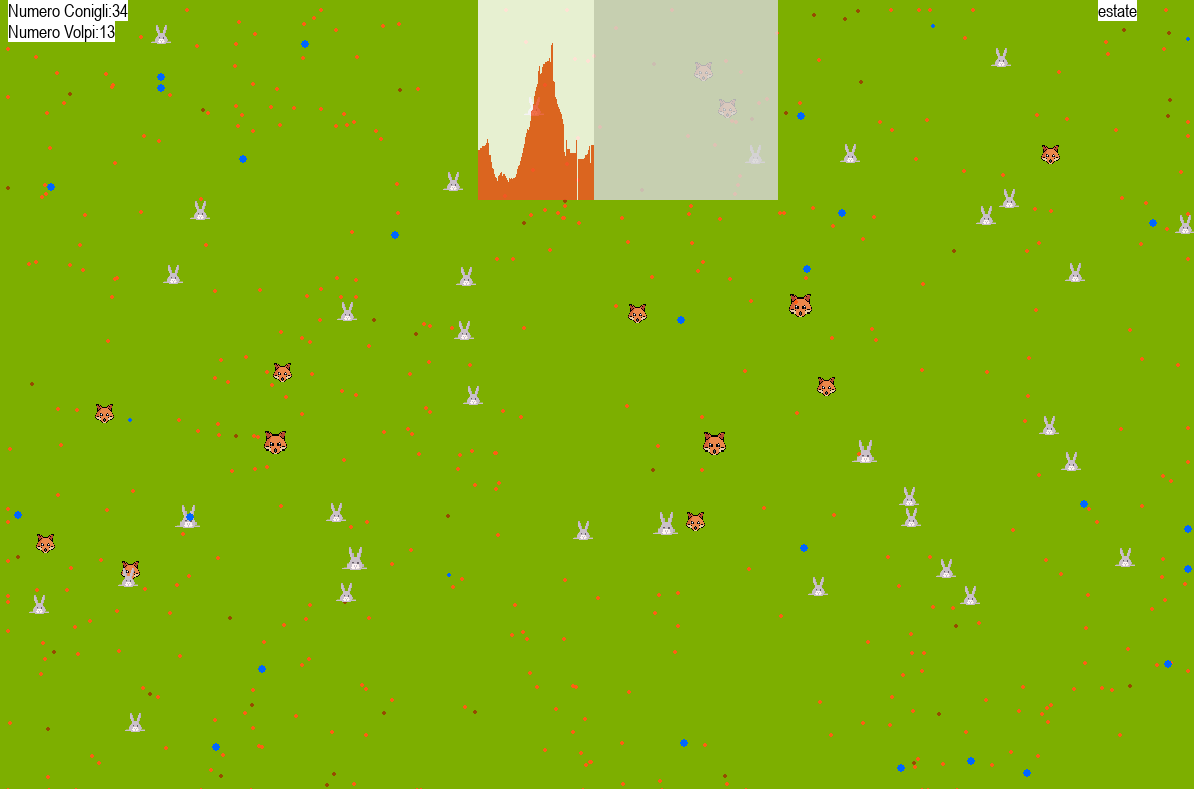
\includegraphics[scale = 0.2]{SIMULAZIONE_Estate.PNG}
        \caption{Estate}
        \label{fig:estate}
	\end{subfigure}
	\caption{Cambi di stagione nella simulazione}
\end{figure}



    \item \textbf{Vector2D}: collezione di metodi per la gestione delle coordinate e dello spazio vettoriale. Vengono utilizzati metodi per ottenere ed elaborare la posizione, la distanza, il modulo (magnitudine), la norma e la direzione dei punti sul piano 2D.
    
    \item \textbf{Plot}: modulo che utilizza come input il file \textit{.csv} generato dalla simulazione e ne visualizza i valori creando diversi grafici e memorizzandoli in cartelle apposite, nominate in modo tale da riportare il seed della simulazione e un tag che identifica la configurazione con cui è stata lanciata la simulazione (tag E significa evoluzione, tag R significa reintroduzione, nessun tag significa che la simulazione è stata lanciata senza reintroduzione e senza evoluzione). I grafici generati per ogni simulazione sono i seguenti:
    \begin{itemize}
        \item \textbf{\textit{conigli-carote.png}}: mostra la differenza tra le popolazioni di conigli e carote;
        \item \textbf{\textit{età.png}}: mostra le differenze dell'età media tra le due specie;
        \item \textbf{\textit{fame.png}}: mostra le differenze di fame media tra le due specie;
        \item \textbf{\textit{sete.png}}: mostra le differenze di sete media tra le due specie;
        \item \textbf{\textit{fertilita.png}}: mostra le differenze di fertilità media tra le due specie;
        \item \textbf{\textit{morti\_conigli.png}}: mostra le cause di morte dei conigli;
        \item \textbf{\textit{morti\_volpi.png}}: mostra le cause di morte delle volpi;
        \item \textbf{\textit{nascite.png}}: mostra le nascite delle due specie a confronto;
        \item \textbf{\textit{popolazioni.png}}: mostra le popolazioni degli animali a confronto;
        \item \textbf{\textit{risorse.png}}: mostra le risorse a confronto;
        \item \textbf{\textit{percezione.png}}: mostra la percezione media degli animali;
        \item \textbf{\textit{soglia\_fame\_media.png}}: mostra la soglia fame media degli animali;
        \item \textbf{\textit{soglia\_sete\_media.png}}: mostra la soglia sete media degli animali;
        \item \textbf{\textit{soglia\_morte\_di\_fame\_media.png}}: mostra la soglia di morte di fame media degli animali;
        \item \textbf{\textit{soglia\_morte\_di\_sete\_media.png}}: mostra la soglia di morte di sete media degli animali;
        \item \textbf{\textit{velocita\_camminata\_media.png}}: mostra la velocità di camminata media degli animali;
        \item \textbf{\textit{velocita\_corsa\_media.png}}: mostra la velocità di corsa media degli animali;
        \item \textbf{\textit{stackedBarchart\_cause\_morti\_volpi.png}}: è uno stacked barchart che mostra come sono suddivise il numero e le cause di morte delle volpi nelle quattro stagioni;
        \item \textbf{\textit{stackedBarchart\_cause\_morti\_conigli.png}}: analogo a quello descritto nel punto precedente, ma relativo ai conigli;
        \item \textbf{\textit{conigliVsVolpi\_NoTimeSeries.png}}: è un grafico che mostra sull'asse delle ascisse il numero di prede e sulle ordinate il numero di predatori. Questo grafico è risultato utile per eseguire la validazione del modello;
        \item \textbf{\textit{caroteVsConigli\_NoTimeSeries.png}}: analogamente a quello del punto precedente, mostra sull'asse delle ascisse il numero di carote e su quello delle ordinate il numero di conigli. Anche questo è risultato utile in fase di validazione del modello.
    \end{itemize}
\end{itemize}


\section{Analisi dei risultati}
Per collezionare i dati ed analizzare i risultati ottenuti, sono state lanciate svariate simulazioni relative a diverse configurazioni del modello. Tra le varie configurazioni testate, le tre principali per le quali è stata condotta un'analisi dei risultati sono le seguenti: 
\begin{itemize}
    \item \textbf{Senza reintroduzione e senza evoluzione};
    \item \textbf{Con reintroduzione e senza evoluzione};
    \item \textbf{Con reintroduzione ed evoluzione};
\end{itemize}

\vspace{1cm}

\subsection{Configurazione senza reintroduzione e senza evoluzione}
La prima configurazione è stata implementata in modo tale che non vi fosse una periodica reintroduzione degli agenti animale nell'ambiente e che non venisse simulata l'evoluzione genetica degli individui, per tale ragione è anche la configurazione più semplice delle tre e quella i cui risultati si sono rivelati essere poco soddisfacenti. Per questo motivo, essa è stata un punto di partenza dalla quale sono state realizzate le configurazioni successive che hanno dato risultati decisamente più attendibili. 
La differenza tra un sistema con reintroduzione e senza reintroduzione riguarda il fatto che nel secondo caso alcuni animali (sia prede che predatori) vengono inseriti all'interno dell'ambiente con una certa frequenza, mentre nel primo caso questa operazione non viene mai eseguita, lasciando quindi l'ambiente totalmente chiuso.

Questa prima configurazione, nonostante gli esiti non siano stati del tutto soddisfacenti, è stata particolarmente utile per effettuare una prima operazione di tuning ottimale dei vari  parametri coinvolti dalla simulazione e descritti nei paragrafi precedenti. Per esempio, si è tentato di trovare una soluzione che permettesse di ottenere un trend verosimile delle cause di morte degli animali, facendo in modo che la frequenza dei decessi causati dalla vecchiaia risultassero inferiori rispetto a quelli dovuti ad altre cause (fame, sete e caccia), che invece sarebbero dovute risultare bilanciate tra loro.   


\begin{figure}[h!]
     \centering
     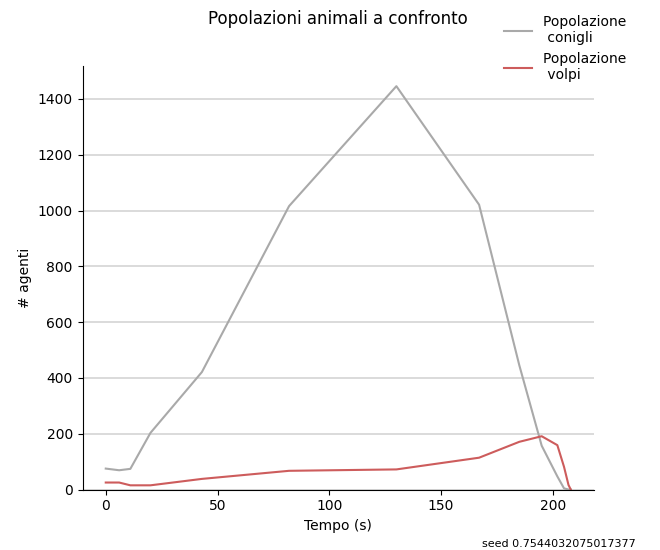
\includegraphics[scale = 0.7]{popolazioniNoReintroduzione.png}
     \caption{Grafico popolazione volpi vs popolazione conigli}
     \label{fig:coniglioVolpeNoReintroduzione}
\end{figure}

Il grafico in \textbf{figura \ref{fig:coniglioVolpeNoReintroduzione}} mostra l'andamento nel tempo delle popolazioni delle prede e dei predatori ottenuto con questa prima configurazione del modello. Si può osservare che i conigli inizialmente crescono notevolmente in numero, ma quando saturano le risorse disponibili nell'ambiente iniziano a morire di fame, e anche a causa della predazione condotta dai predatori, la popolazione si estingue e di conseguenza anche il numero di volpi tende a decrescere fino a quando non si estinguono anch'esse, a causa della mancanza di prede di cui cibarsi. Possiamo quindi concludere che il modello è risultato essere instabile, in quanto, in quasi tutte le esecuzioni, si è verificata l'estinzione di entrambe le specie di animali.


\begin{figure}[h!]
	\begin{subfigure}{\textwidth}
            \centering
            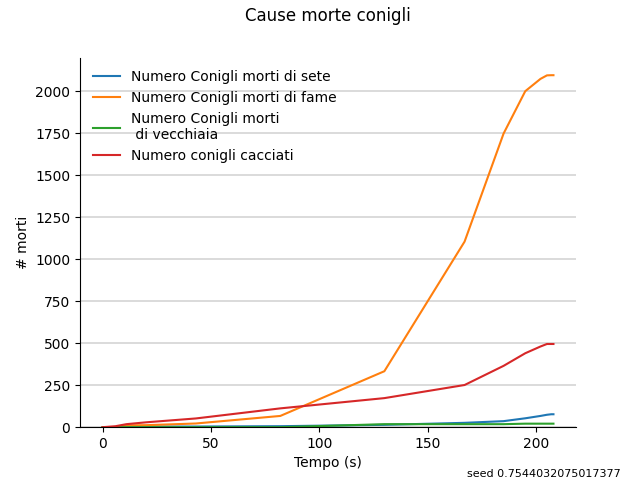
\includegraphics[scale = 0.75]{mortiConigliNoReintroduzione.png}
            \caption{Cause morte dei conigli}
            \label{fig:morteConigliNoReintroduzione}
	\end{subfigure}
		\begin{subfigure}{\textwidth}
		\centering
        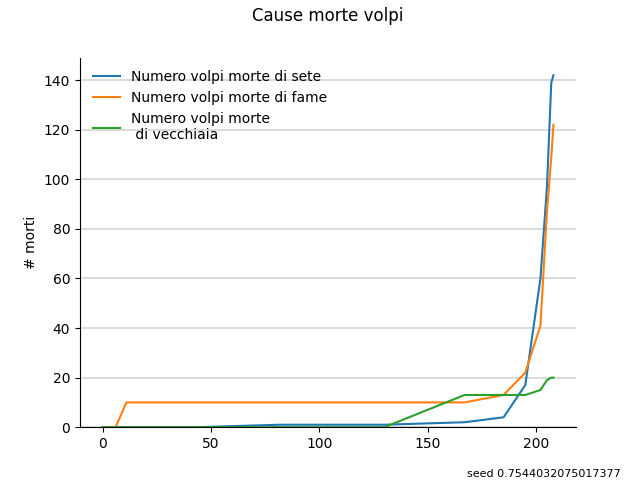
\includegraphics[scale = 0.75]{mortiVolpiNoReintroduzione.png}
        \caption{Cause morte delle volpi}
        \label{fig:morteVolpeNoReintroduzione}
	\end{subfigure}
\caption{Grafici cause morte degli animali}
\end{figure}

\newpage

I grafici \textbf{\ref{fig:morteConigliNoReintroduzione}} e \textbf{\ref{fig:morteVolpeNoReintroduzione}}  mostrano lo sviluppo nel tempo delle cause di morte, rispettivamente delle prede e dei predatori. Si può notare che la causa di morte prevalente nella popolazione dei conigli è la fame, seguita dalla caccia da parte delle volpi. A causa della brevità della simulazione, un numero molto basso di conigli tende a morire di sete. Per lo stesso motivo solamente 21 conigli sono risultati morti di vecchiaia nell'esecuzione mostrata nei grafici riportati. 

Per quanto riguarda le volpi, le cause di morte più frequenti sono risultate essere la sete e la fame. Il numero di volpi morte di vecchiaia è risultato essere uguale a quello dei conigli morti per lo stesso motivo. 



\noindent Come è possibile notare dalle \textbf{figure \ref{fig:coniglioVolpeNoReintroduzione}}, \textbf{\ref{fig:morteConigliNoReintroduzione}} e \textbf{\ref{fig:morteVolpeNoReintroduzione}}, il tempo di esecuzione della simulazione è molto basso, infatti si conclude in poco più di 200 secondi. Il sistema infatti, risulta essere piuttosto instabile in quanto gli animali tendono ad estinguersi completamente dopo poco tempo dall'inizio della simulazione. 
Per andare oltre questo problema, si è deciso di estendere ulteriormente il modello realizzando un approccio alternativo con reinserimento, i cui risultati sono esposti nella sezione successiva. 

\clearpage
\newpage


\subsection{Configurazione con reintroduzione senza evoluzione}
\label{sec:reintroduzioneNoEvoluzione}
L'idea di questa configurazione è quella di non pensare più all'ambiente come una scatola chiusa, ma far si che ci sia la possibilità che nuovi animali (sia volpi che conigli) possano entrare nell'ambiente dall'esterno, in modo tale da simulare le migrazioni di animali dalle aree circostanti, come se lo spazio che viene visualizzato sia una piccola porzione posizionata in un ambiente più grande. 
Seguendo questa logica, è stato fatto in modo che, ogni qualvolta si verifica un cambio di stagione durante la simulazione, venissero inseriti volpi e conigli nell'ambiente in numero proporzionale rispetto alla quantità di animali presenti all'inizio della simulazione stessa.


\begin{figure}[h!]
	\hspace{-5mm}
	\begin{subfigure}{\textwidth}
            \centering
     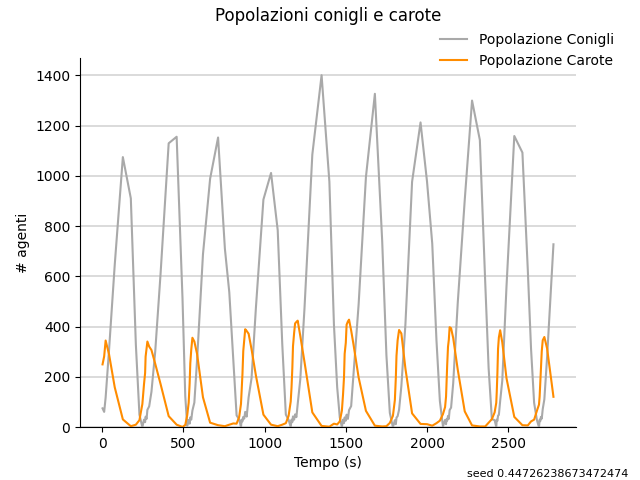
\includegraphics[scale = 0.52]{conigli-caroteR.png}
     \caption{Grafico popolazione conigli vs popolazione carote}
     \label{fig:conigliCaroteReintroduzione}
	\end{subfigure}
	\begin{subfigure}{\textwidth}
		\centering
     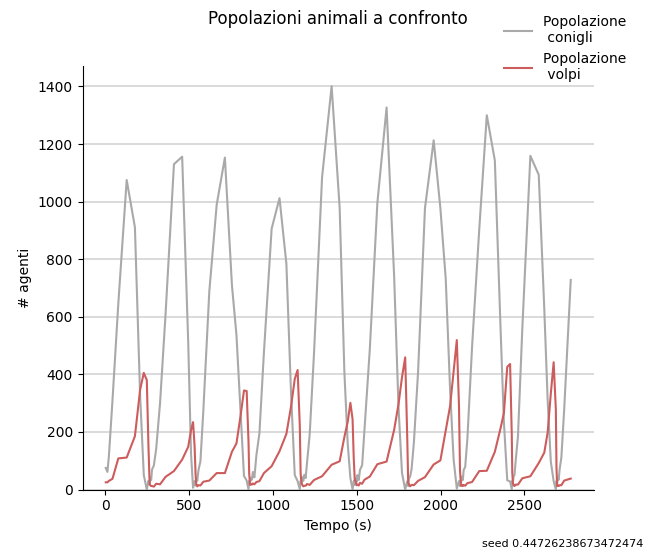
\includegraphics[scale = 0.52]{popolazioniR.png}
     \caption{Grafico popolazione conigli vs popolazione volpi}
     \label{fig:conigliVolpiReintroduzione}
	\end{subfigure}
\end{figure}

\newpage

Dal \textbf{grafico \ref{fig:conigliCaroteReintroduzione}} è possibile notare innanzitutto che il sistema così esteso risulta essere stabile, a differenza del modello nella configurazione presentata in precedenza, in quanto non si verifica mai durante la simulazione l'estinzione di tutti gli animali. 
Il numero delle carote e dei conigli presenti nel sistema segue un andamento di questo tipo: inizialmente i conigli crescono in numero, fino a diventare circa 1100 e contemporaneamente le carote vengono completamente mangiate fino a quando non ne resta praticamente nessuna; a questo punto il numero di conigli inizia a diminuire drasticamente a causa del fatto che nell'ambiente non è presente abbastanza cibo per poter sostentare tutta la popolazione. Nel contempo, il numero di carote inizia a crescere e all'incirca quando il numero di conigli ha raggiunto il minimo locale, esso raggiunge il massimo. Dopodiché, il numero di conigli può tornare a crescere, dato che ci sono abbastanza carote nell'ambiente. Tutto ciò si ripete ciclicamente fino al termine della simulazione. 

La \textbf{figura \ref{fig:conigliVolpiReintroduzione}} mostra invece l'andamento delle popolazioni dei conigli e delle volpi nel corso della simulazione. Come si vede dall'immagine, il trend è esattamente analogo a quello delle popolazioni dei conigli e delle carote discusso in precedenza. In entrambi i casi infatti, l'andamento segue all'incirca quello di due sinusoidi sfasate che si ripetono ciclicamente.


\begin{figure}[h!]
     \centering
     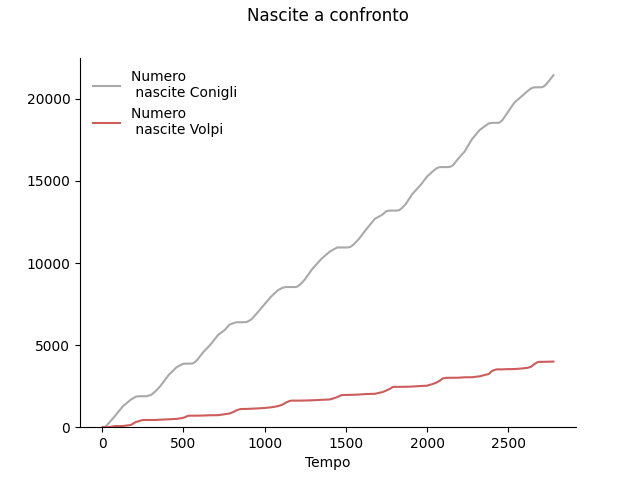
\includegraphics[scale = 0.6]{nasciteR.png}
     \caption{Grafico delle nascite dei conigli e delle volpi}
     \label{fig:nasciteReintroduzione}
\end{figure}



La \textbf{figura \ref{fig:nasciteReintroduzione}} mostra come evolvono le nascite all'interno delle due popolazioni. Come, prevedibile, è risultato che i conigli si riproducono con una frequenza significativamente superiore rispetto alle volpi. 

\newpage

\begin{figure}[!ht]
	\begin{subfigure}{\textwidth}
         \centering
         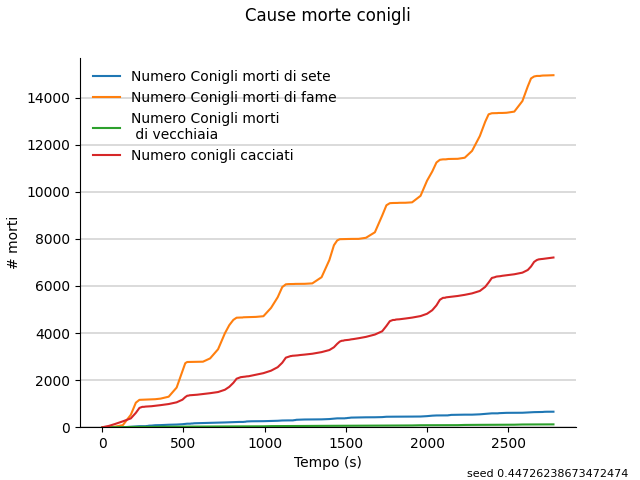
\includegraphics[scale = 0.6]{morti_conigliR.png}
         \caption{Cause di morte conigli}
         \label{fig:morteConigliReintroduzione}
	\end{subfigure}
	\begin{subfigure}{\textwidth}
		\centering
        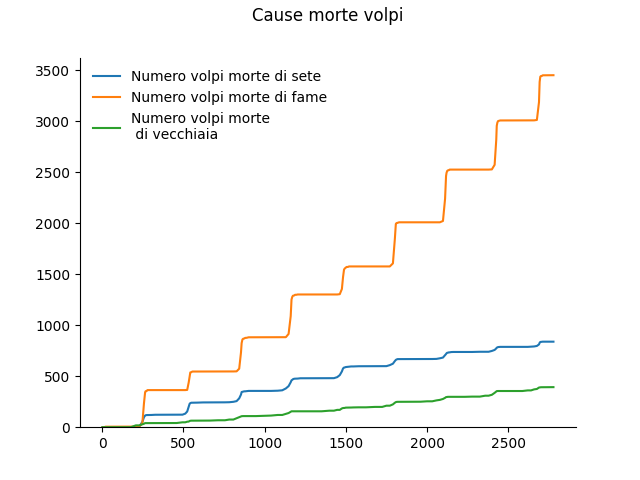
\includegraphics[scale = 0.6]{morti_volpiR.png}
        \caption{Cause di morte volpi}
        \label{fig:morteVolpiReintroduzione}
	\end{subfigure}
	\caption{Grafici cause di morte animali}
\end{figure}


Il \textbf{grafico \ref{fig:morteConigliReintroduzione}} mostra l'andamento del numero di decessi dei conigli suddivisi in base alla causa. Si può notare che anche in questo caso i conigli muoiono perlopiù di fame a causa del fatto che, come appurato dal grafico mostrato in \textbf{figura \ref{fig:nasciteReintroduzione}}, essi tendono a riprodursi frequentemente e quindi questo porta alla competizione tra gli individui per ottenere le carote disponibili. Molto rilevante è anche il numero di morti causate dalla caccia da parte dei predatori. Invece, il numero di conigli morti di sete e di vecchiaia risulta essere piuttosto contenuto. 

Dalla \textbf{figura \ref{fig:morteVolpiReintroduzione}}, che rappresenta il grafico relativo all'andamento delle numero di decessi delle volpi e le loro cause, si può notare che anche in questo caso la causa di morte prevalente tra le volpi è la fame. Questo perché nei momenti in cui sono presenti pochi conigli nell'ambiente le volpi non trovano prede con cui sfamarsi e di conseguenza muoiono. La seconda causa più rilevante è la sete e infine vecchiaia. La ragione per la quale sia per le volpi che per i conigli la vecchiaia sia solo l'ultima delle cause di morte è che gli individui di entrambe le popolazioni difficilmente riescono a raggiungere l'età della vecchiaia perché tendenzialmente muoiono prima a causa della scarsità delle risorse (acqua per entrambe le specie, carote per i conigli e conigli per le volpi) che si verifica ciclicamente nella simulazione. 



\begin{figure}[!ht]
     \centering
     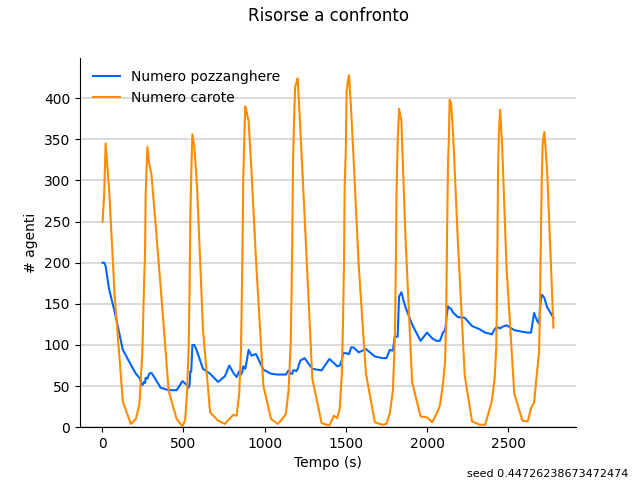
\includegraphics[scale = 0.75]{risorseR.png}
     \caption{Grafico delle risorse}
     \label{fig:risorseReintroduzione}
\end{figure}


Oltre a ciò, dal grafico in \textbf{figura \ref{fig:risorseReintroduzione}} si può notare che il numero di pozzanghere presenti nell'ambiente rimane sempre abbastanza equilibrato a differenza delle carote che tendono a esaurirsi in modo ciclico. É questa la ragione per cui gli individui di entrambe le popolazioni raramente muoiono di sete.

\newpage

\begin{figure}[!ht]
    \hspace{-1.7cm}
     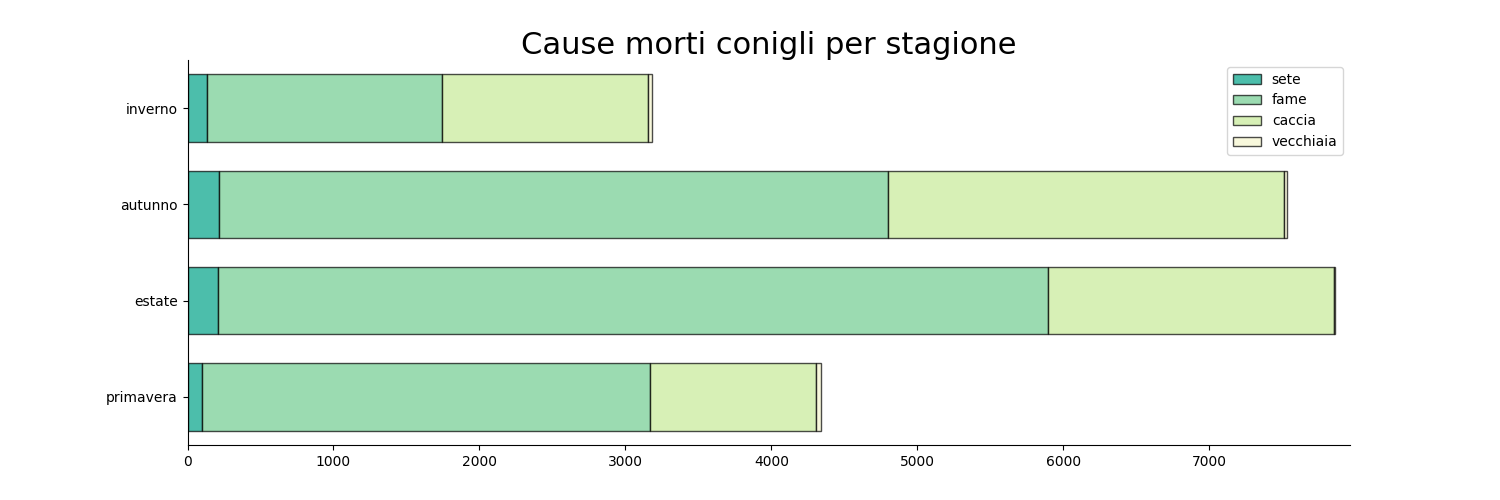
\includegraphics[scale = 0.45]{stackedBarchart_cause_morti_conigli_R.png}
     \caption{Barchart delle morti dei conigli}
     \label{fig:barchartConigliR}
\end{figure}
\begin{figure}[!ht]
    \hspace{-1.7cm}
     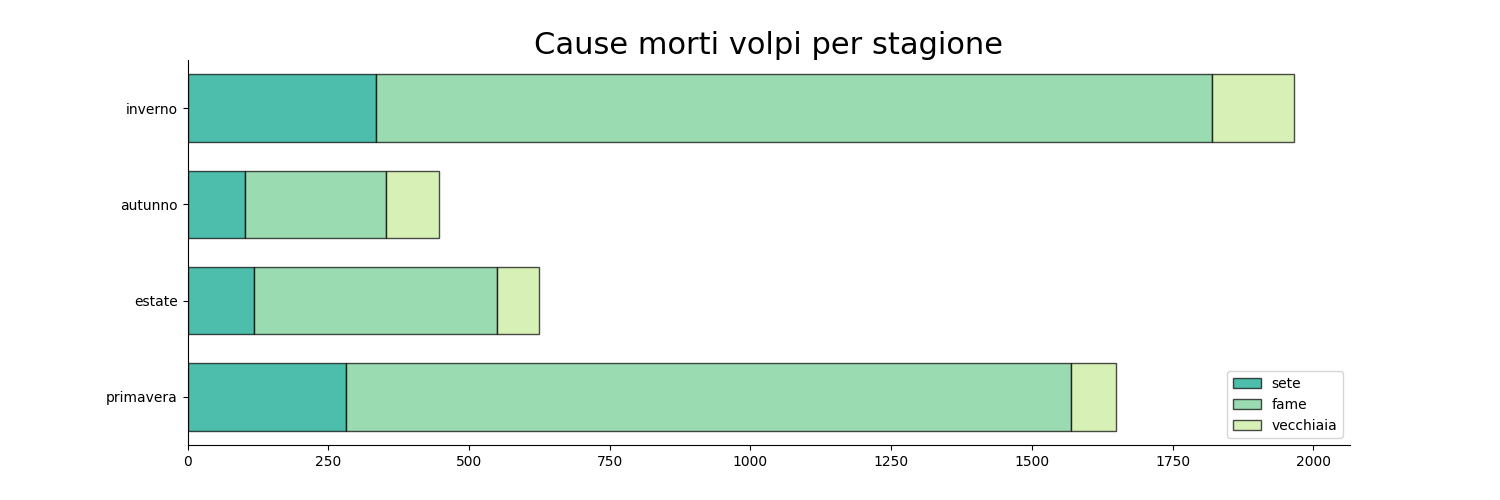
\includegraphics[scale = 0.45]{stackedBarchart_cause_morti_volpi_R.png}
     \caption{Barchart delle morti delle volpi}
     \label{fig:barchhartVolpiR}
\end{figure}

Infine, i grafici mostrati nelle \textbf{figure \ref{fig:barchartConigliR}} e \textbf{\ref{fig:barchhartVolpiR}} indicano come sono ripartite le morti, rispettivamente dei conigli e delle volpi, rispetto alle stagioni. I decessi dei conigli avvengono prevalentemente in autunno e in estate e la causa principale è la mancanza di cibo. Le volpi invece tendono a morire prevalentemente in inverno e in primavera e anche in questo caso la causa principale riguarda la mancanza di prede di cui cibarsi. Una possibile spiegazione riguarda il fatto che, come analizzato, i conigli tendono a morire perlopiù in autunno e in estate, quindi il numero di prede presenti nell'ambiente tende a calare in queste stagioni. L'effetto sui predatori però non è immediato, ma inizia a presentarsi solo nelle stagioni successive in inverno e in primavera quando il numero di morti delle volpi a causa della mancanza di prede cresce in modo notevole rispetto alle altre due stagioni.  


\newpage


\subsection{Configurazione con reintroduzione ed evoluzione}

\begin{figure}[h!]
	\begin{subfigure}{\textwidth}
    \centering
     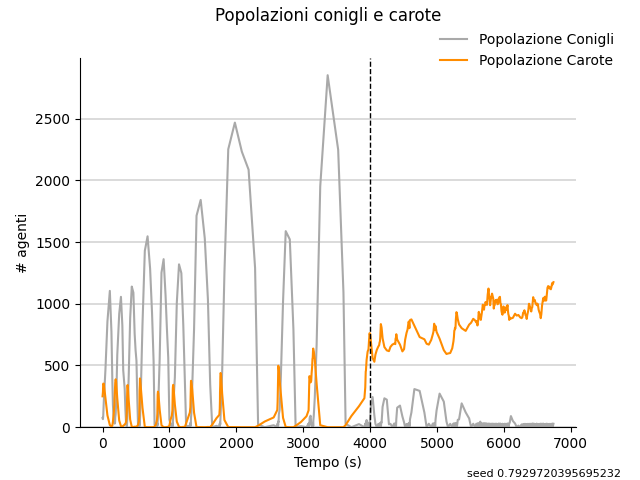
\includegraphics[scale = 0.7]{conigli-carote_RE.png}
     \caption{Popolazione conigli vs popolazione carote}
     \label{fig:conigliCaroteRE}
	\end{subfigure}
	\begin{subfigure}{\textwidth}
		\centering
     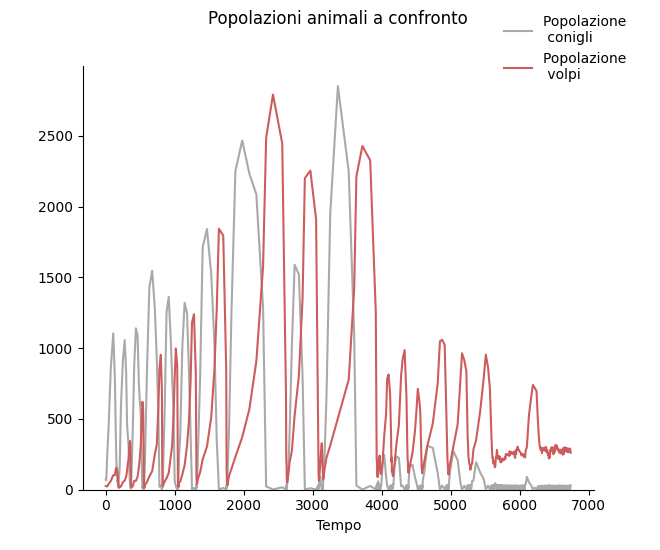
\includegraphics[scale = 0.7]{popolazioni_RE.png}
     \caption{Popolazione conigli vs popolazione volpi}
     \label{fig:conigliVolpiRE}
	\end{subfigure}
	 \caption{Grafici delle popolazioni}
\end{figure}

\newpage
\noindent Questa configurazione consente di effettuare un ulteriore passo avanti, in quanto permette di simulare anche l'evoluzione genetica negli animali. L'obiettivo è stato quello di verificare se l'aggiunta di un fenomeno di mutazione delle caratteristiche degli animali potesse in qualche modo cambiare l'esito della simulazione, e quindi l'equilibrio dell'ecosistema. Per rendere compatibile il processo evolutivo con il reinserimento, è stato assunto che gli animali al di fuori dell'ambiente visualizzato subiscano la stessa pressione evolutiva di quelli visualizzati nell'ambiente simulato. Di conseguenza, ogni volta che vi è reintroduzione, i parametri dei nuovi animali inseriti nell'ambiente saranno uguali alla media di quelli degli animali già presenti nello spazio simulato, portando così avanti il fenomeno di selezione naturale. Questa configurazione rappresenta il modello finale e più complesso delle tre analizzate e quello che ha portato ai risultati più interessanti e significativi.



L'andamento della simulazione nel tempo può essere suddiviso in due fasi, che nei grafici di seguito sono state evidenziate attraverso una linea verticale tratteggiata. Il primo stadio, che nei grafici va dall'inizio a circa l'istante 4000 della simulazione, vede i conigli sfruttare l'unica "arma" a loro disposizione per contrastare il dominio delle volpi, ovvero la loro elevata capacità riproduttiva, come mostrato chiaramente nella \textbf{figura \ref{fig:fertilitaRE}}. I conigli tendono ad evolvere abbassando drasticamente la loro soglia di fertilità, in modo tale che si verifichi un'esplosione di nascite che permette alla popolazione delle prede di contrastare la capacità predatoria delle volpi. Come possibile notare nella \textbf{figura \ref{fig:conigliVolpiRE}}, questo porta ad una situazione nella quale i conigli risultano essere in netta maggioranza rispetto alle volpi, raggiungendo picchi di quasi 3000 individui. Ciò però comporta anche diversi malus per i conigli stessi. Infatti, questa situazione porta ad una rapida saturazione delle risorse (\textbf{figura \ref{fig:conigliCaroteRE}}) e ad un aumento del numero di volpi proporzionale, se pur più lento, a quello dei conigli. In questo modo, viene garantita alle volpi l'energia necessaria per poter continuare a riprodursi. \\
La seconda fase, che inizia dall'istante 4000 e si prolunga fino al termine della simulazione, invece è caratterizzata da un dominio delle volpi nell'ambiente. Esse infatti, acquisiscono un controllo territoriale totale. Questo è dovuto al fatto che i predatori, col passare del tempo, migliorano costantemente le loro caratteristiche, fino ad ottenere un vantaggio rispetto alle prede tale che molte di esse vengono cacciate prima che si possano riprodurre. Questo, come mostra la \textbf{figura \ref{fig:nasciteRE}}, produce un rallentamento nelle nascite dei conigli. Tuttavia, nel lungo periodo, a causa del ridotto numero di prede presenti nell'ambiente, la crescita del numero di volpi subirà una frenata, producendo come effetto un nuovo equilibrio tra le due specie.

\newpage

\begin{figure}[h!]
	\hspace{-8mm}
	\begin{subfigure}{.5\textwidth}
         \centering
         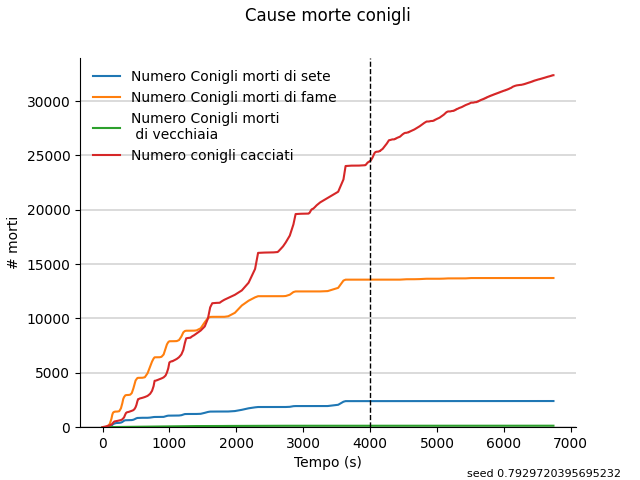
\includegraphics[scale = 0.5]{morti_conigli_RE.png}
         \caption{Grafico cause di morte conigli}
         \label{fig:morteConigliRE}
	\end{subfigure}
	\begin{subfigure}{.5\textwidth}
		\hspace{7mm}
		\centering
        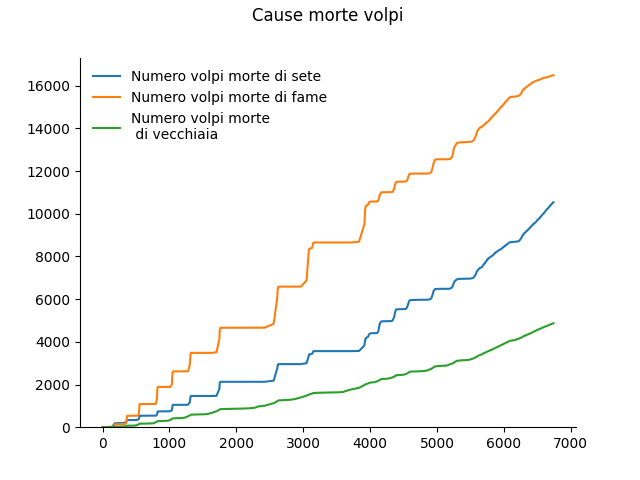
\includegraphics[scale = 0.5]{morti_volpi_RE.png}
        \caption{Grafico cause di morte volpi}
        \label{fig:morteVolpiRE}
	\end{subfigure}

	\hspace{-8mm}
	\begin{subfigure}{.5\textwidth}
         \centering
         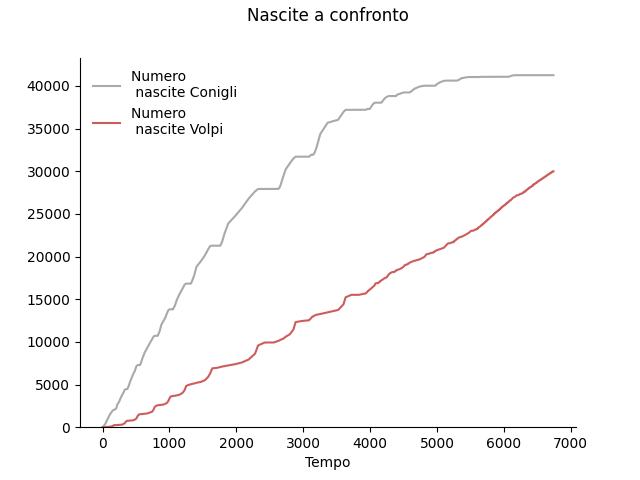
\includegraphics[scale = 0.5]{nascite_RE.png}
         \caption{Grafico nascite a confronto}
         \label{fig:nasciteRE}
	\end{subfigure}
	\begin{subfigure}{.5\textwidth}
		\hspace{7mm}
		\centering
        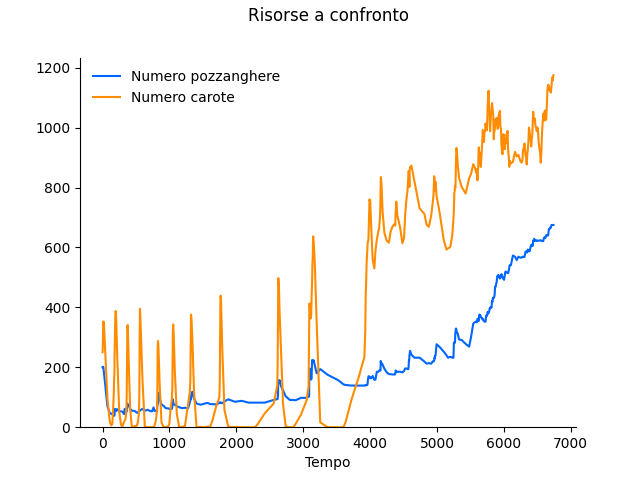
\includegraphics[scale = 0.5]{risorse_RE.png}
        \caption{Grafico risorse a confronto}
        \label{fig:risorseRE}
	\end{subfigure}
	 \caption{}
\end{figure}


\begin{itemize}


    \item La \textbf{figura \ref{fig:morteConigliRE}} mostra come le cause di morte dei conigli inizialmente siano bilanciate tra fame e caccia. Però quest'ultima diventa predominante nella seconda fase della simulazione nella quale le volpi prendono il sopravvento sui conigli. La \textbf{figura \ref{fig:morteVolpiRE}} mostra invece come le cause di morte relative alle volpi siano bilanciate tra loro. Nella fase iniziale è possibile notare dei "salti" relativi ai momenti in cui i conigli proliferano e momenti in cui la mancanza di prede e acqua, porta a un elevato numero di decessi nella popolazione delle volpi.


    \item La \textbf{figura \ref{fig:nasciteRE}} mostra chiaramente la dicotomia tra le due fasi; la prima in cui i conigli si diffondono vertiginosamente e la seconda in cui si arriva ad un punto asintotico in cui il numero delle nascite degli stessi subisce un forte rallentamento dovuto all'evoluzione delle caratteristiche delle volpi.


    \item La \textbf{figura \ref{fig:risorseRE}} mostra una prima fase di carenza di carote e pozzanghere presenti nell'ambiente e una seconda in cui l'assenza dei conigli comporta una crescita costante delle stesse.

\end{itemize}

\begin{figure}[h!]
	\begin{subfigure}{\textwidth}
         \centering
         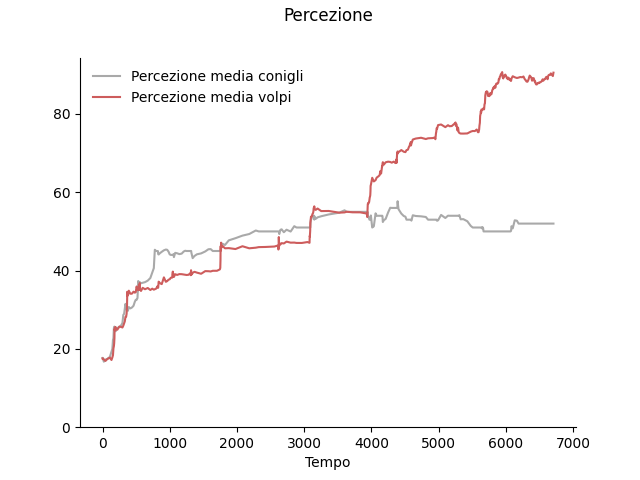
\includegraphics[scale = 0.55]{Percezione_RE.png}
         \caption{Grafico andamento della caratteristica percezione media}
         \label{fig:percezioneRE}
	\end{subfigure}
	\begin{subfigure}{\textwidth}
		\centering
        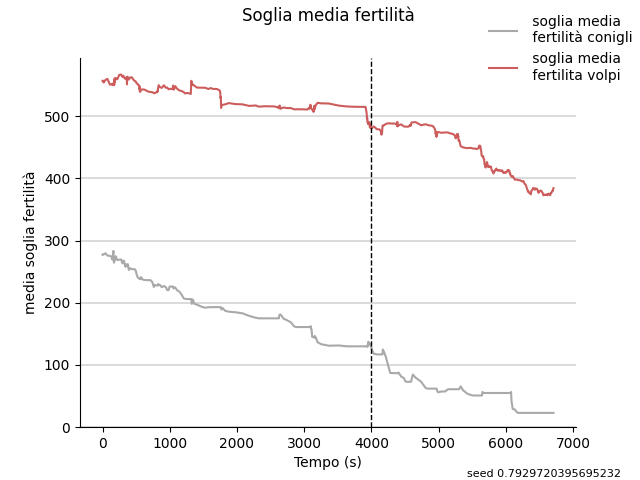
\includegraphics[scale = 0.55]{soglia_fertilita_media_RE.png}
        \caption{Grafico andamento della caratteristica soglia fertilità media}
        \label{fig:fertilitaRE}
	\end{subfigure}
\end{figure}

\begin{itemize}


    \item La \textbf{figura \ref{fig:percezioneRE}} mostra quanto l'evoluzione giochi un ruolo fondamentale in questo modello. Le volpi arrivano a quadruplicare la loro percezione base, andando ad ottenere un controllo sul territorio molto più esteso.

    \item La \textbf{figura \ref{fig:fertilitaRE}} mostra come tra le due popolazioni sia quella dei conigli a trarre un enorme vantaggio dall'abbassamento della soglia di fertilità. Il valore medio, negli ultimi istanti della simulazione, addirittura sfiora lo zero, confermando quanto sia importante per i conigli questa caratteristica per contrastare il diffondersi dei predatori nel territorio. 
\end{itemize}

\newpage

\begin{figure}[h!]
	\begin{subfigure}{\textwidth}
         \centering
         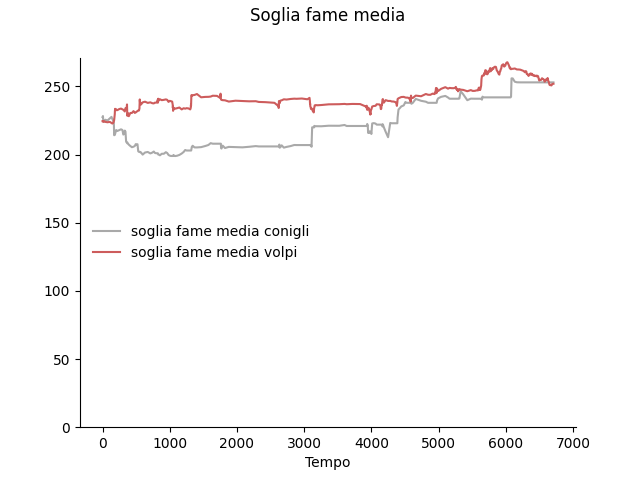
\includegraphics[scale = 0.60]{soglia_fame_media_RE.png}
         \caption{Grafico andamento della caratteristica soglia fame media}
         \label{fig:FameRE}
	\end{subfigure}
	\begin{subfigure}{\textwidth}
		\centering
        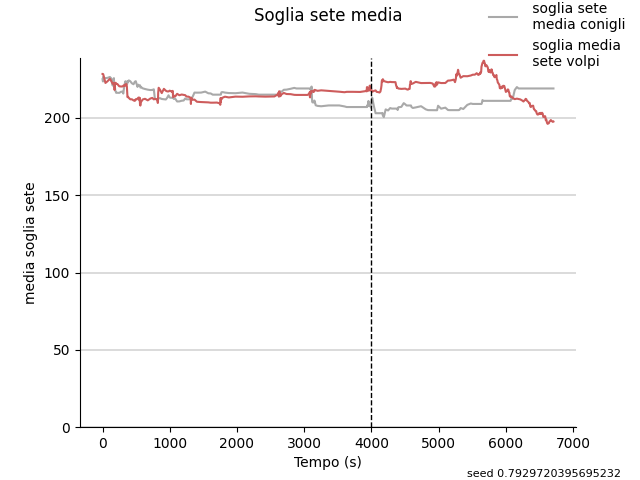
\includegraphics[scale = 0.60]{soglia_sete_media_RE.png}
        \caption{Grafico andamento della caratteristica soglia sete media}
        \label{fig:SeteRE}
	\end{subfigure}
	\caption{}
\end{figure}

\begin{itemize}


    \item Le \textbf{figure \ref{fig:FameRE}} e \textbf{\ref{fig:SeteRE}} sono simili e mostrano un dato interessante: le soglie di fame e sete non hanno un grande peso nell'evoluzione degli animali. Questo probabilmente è dovuto al fatto che all'inizio della simulazione le due soglie degli individui di entrambe le popolazioni assumono valori piuttosto bassi e quindi un'ulteriore diminuzione delle stesse non porta un vantaggio evolutivo significativo.
\end{itemize}

\newpage 

\begin{figure}[ht!]
	\hspace{-2mm}
	\begin{subfigure}{\textwidth}
         \centering
         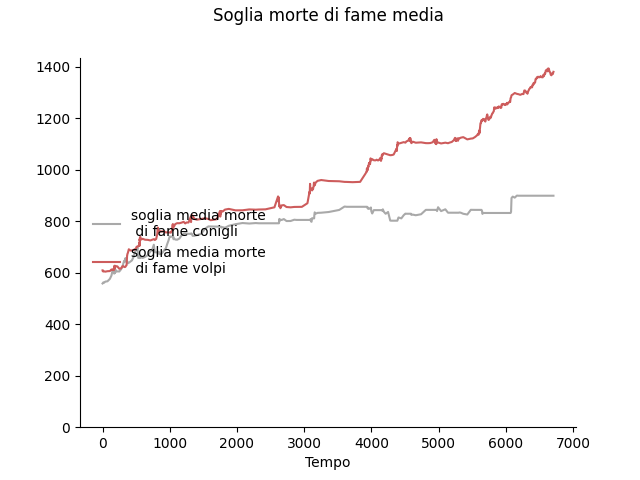
\includegraphics[scale = 0.60]{soglia_morte_di_fame_media_RE.png}
         \caption{Grafico andamento della caratteristica soglia morte di fame media}
         \label{fig:morteFameRE}
	\end{subfigure}
	\begin{subfigure}{\textwidth}
		\centering
        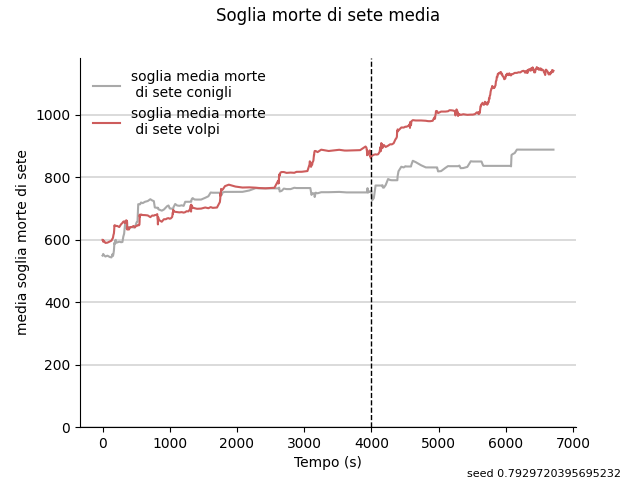
\includegraphics[scale = 0.60]{soglia_morte_di_sete_media_RE.png}
        \caption{Grafico andamento della caratteristica soglia morte di sete media}
        \label{fig:morteSeteRE}
	\end{subfigure}
	\caption{}
\end{figure}



\begin{itemize}


    \item Le \textbf{figure \ref{fig:morteFameRE}} e \textbf{\ref{fig:morteSeteRE}} sono altrettanto equiparabili e mostrano come le soglie di morte di fame e di sete invece, siano caratteristiche che, tramite l'evoluzione, possono permettere agli individui di adattarsi meglio all'ambiente permettendogli di sopravvivere più a lungo. Saranno gli agenti che hanno una maggiore resistenza alle carenze di risorse, quelli che si adatteranno meglio e che quindi avranno più possibilità di sopravvivere e trasmettere alla prole questa caratteristica. 
    
\end{itemize}

\newpage 

\begin{figure}[ht!]
	\begin{subfigure}{\textwidth}
         \centering
         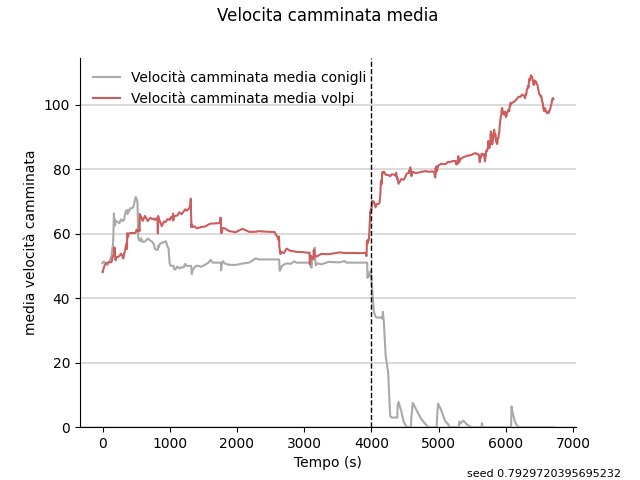
\includegraphics[scale = 0.77]{velocita_camminata_media_RE.png}
         \caption{Grafico andamento della caratteristica velocità camminata media}
         \label{fig:camminataRE}
	\end{subfigure}
	\begin{subfigure}{\textwidth}
		\centering
        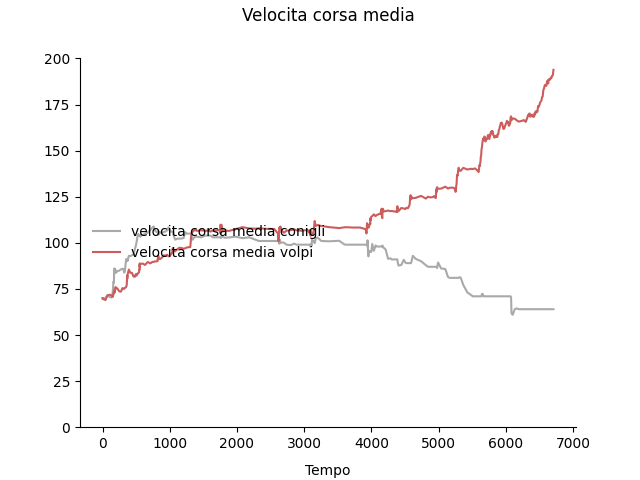
\includegraphics[scale = 0.77]{velocita_corsa_media_RE.png}
        \caption{Grafico andamento della caratteristica velocità corsa media}
        \label{fig:corsaRE}
	\end{subfigure}
\caption{}
\end{figure}

\begin{itemize}


    \item Le \textbf{figure \ref{fig:camminataRE}} e \textbf{\ref{fig:corsaRE}} rappresentano i risultati più sorprendenti. E' possibile notare come, se nella prima parte della simulazione i valori non subiscano cambiamenti significativi rispetto alle velocità di corsa e di camminata, nella seconda invece, si crei una vera e propria divergenza tra lo stesso parametro nelle popolazioni delle due specie. Una possibile interpretazione relativa a questa differenza è la seguente:
    \begin{itemize}
        \item Le volpi, dopo aver sovrastato in numero la popolazione delle prede, hanno a disposizione pochi conigli di cui cibarsi e dunque questo determina il fatto che saranno gli esemplari più veloci quelli che riusciranno a raggiungere con più facilità le poche prede rimaste, evitando così di morire di fame. In altre parole, il principio di selezione naturale favorirà gli individui più rapidi, che saranno facilitati nel catturare le prede. 
        \item I conigli invece, in situazione di netto svantaggio rispetto ai predatori, comprendono che la soluzione migliore sia quella di muoversi il meno possibile, evitando di esporsi alle minacce. Infatti, si nota come la velocità di corsa rimanga stabile, ma la loro velocità di camminata tende a decrescere sempre più. Questo significa che i conigli a lungo termine tendono a evitare di effettuare movimenti, a meno che non ci sia un obiettivo nelle immediate vicinanze. Questo può essere interpretato come un modo per i conigli di nascondersi dai predatori, proprio come nella realtà fanno attraverso l'utilizzo di tane. È proprio questo comportamento a dare il nome a questi mammiferi.\footnote{La parola coniglio deriva da dal latino "\textit{cuniculus}", cioè buca sotterranea.\cite{WikiConiglio} }. 
    \end{itemize}

\end{itemize}

\newpage

\subsubsection{Validazione del modello}
Al fine di verificare che il modello realizzato corrispondesse a ciò che ci si attendeva, è stata eseguita una operazione di validazione dello stesso, descritta in questo paragrafo.
Il modello preso in considerazione per questa fase è quello con reintroduzione senza evoluzione, descritto nella sezione \ref{sec:reintroduzioneNoEvoluzione}. 
Le ragioni per le quali si è deciso di effettuare la validazione solo per questa configurazione sono le seguenti:
\begin{itemize}
    \item Una assunzione di gran parte dei modelli presenti in letteratura, e in particolare del modello Lotka-Volterra, è che gli individui che popolano l'ambiente non subiscano alcun tipo di evoluzione. Per questa ragione si è deciso di effettuare questa operazione solo per il modello più completo tra i tre realizzati che non prevede la simulazione dell'evoluzione;
    \item Gli effetti dell'evoluzione genetica in natura sono riscontrabili solo dopo un lunghissimo periodo di tempo. La creazione di un modello di simulazione che tiene conto dell'evoluzione è quindi una semplificazione di un modello a lunghissimo termine. In letteratura non esistono dati di osservazioni di evoluzioni genetiche a lungo termine con cui poter eseguire un confronto rispetto ai dati ottenuti con la simulazione.
\end{itemize}
Per effettuare questo lavoro sono stati considerati i risultati del modello lotka-volterra, descritto nella sezione \ref{sec:LV}. Oltre a ciò, è stato preso in considerazione anche un set di dati relativi all'interazione della popolazione delle linci canadesi e quella delle lepri scarpa di neve (Lepus americanus), raccolti grazie alle osservazioni durate quasi un secolo condotte dalla Hudson Bay Company\cite{HareLynxData}.  

Per prima cosa, è possibile affermare che il modello nella seconda configurazione risulta essere stabile e la sua esecuzione viene portata avanti per un tempo indefinito senza interrompersi, a differenza del modello realizzato nella prima configurazione.

\begin{figure}[h!]
     \centering
     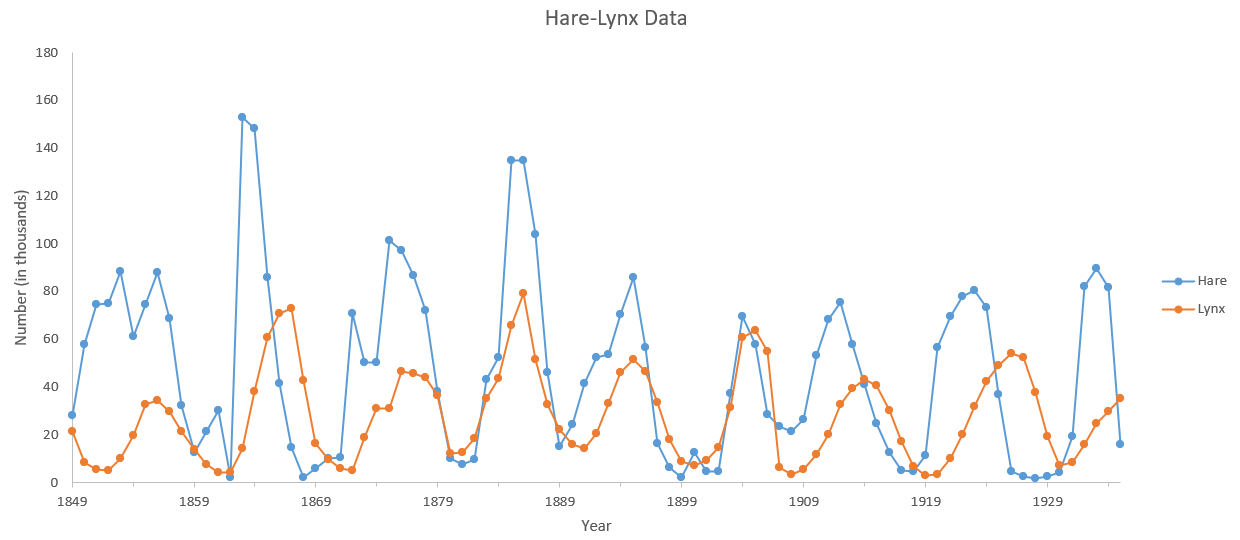
\includegraphics[scale = 0.5]{hareLynx.png}
     \caption{Grafico dell'andamento del numero di individui delle popolazioni di linci canadesi e di lepri scarpa di neve}
     \label{fig:hareLynx}
\end{figure}

La \textbf{figura \ref{fig:hareLynx}} mostra l'evoluzione delle popolazioni delle linci canadesi e delle lepri scarpa di neve, osservate dalla Hudson Bay Company\cite{HareLynx}. Confrontando tale grafico con quelli presentati in precedenza nelle\textbf{ figure \ref{fig:conigliCaroteReintroduzione}} e \textbf{\ref{fig:conigliVolpiReintroduzione}}, si nota che l'andamento è molto simile. Infatti, inizialmente il numero di prede è superiore al numero di predatori, successivamente dopo un momento in cui il numero di predatori cala ulteriormente, esso  tende a risalire e contemporaneamente il numero di prede cala. In seguito il numero di predatori torna a calare e le prede aumentano in numero. Questo pattern si ripete in modo abbastanza sistematico per tutta la durata delle osservazioni. 

\begin{figure}[h!]
     \centering
     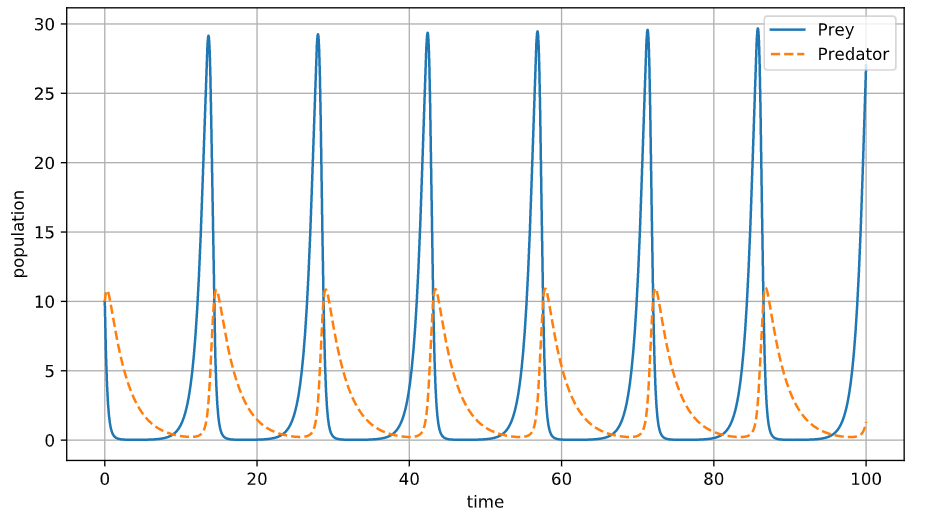
\includegraphics[scale = 0.5]{LV.png}
     \caption{Grafico che mostra la dinamica delle popolazioni preda e predatore simulata mediante il modello Lotka-Volterra}
     \label{fig:LVValidazione}
\end{figure}

La \textbf{figura \ref{fig:LVValidazione}} mostra la dinamica delle popolazioni di specie di predatori e di una di prede che seguono le equazioni di Lotka-Volterra, dati i seguenti parametri: 
\begin{itemize}
	\item numero di prede all'inizio della simulazione: 10;
	\item numero di predatori all'inizio della simulazione: 10;
	\item tasso di crescita delle prede: 1.1;
	\item tasso di morte delle prede: 0.4;
	\item tasso di crescita dei predatori: 0.1;
	\item tasso di morte dei predatori: 0.4
\end{itemize}
Confrontando i \textbf{grafici \ref{fig:conigliCaroteReintroduzione}} e \textbf{\ref{fig:conigliVolpiReintroduzione}} si può notare che l'andamento delle popolazioni del modello da validare e di quelle del modello di Lotka-Volterra sono del tutto speculari. 


\begin{figure}[h!]
	\hspace{-5mm}
	\begin{subfigure}{.5\textwidth}
    \centering
     \includegraphics[scale = 0.50]{fasiLV.png}
     \caption{Grafico Lotka-Volterra}
     \label{fig:LVPhaseSpace}
	\end{subfigure}
	\begin{subfigure}{.5\textwidth}
		\hspace{10mm}
		\centering
     \includegraphics[scale = 0.37]{conigliVSVolpi.png}
     \caption{Grafico modello reinserimento}
     \label{fig:conigliVolpi}
	\end{subfigure}
	\caption{Confronto tra il phase space plot del modello Lotka-Volterra in condizioni diverse in base al numero iniziale di predatori e il grafico popolazione conigli vs popolazione volpi del modello in configurazione con reintroduzione}
\end{figure}
\begin{figure}[h!]
     
\end{figure}

\newpage 

La \textbf{figura \ref{fig:LVPhaseSpace}} mostra sull'asse delle ascisse il numero di prede e sull'asse delle ordinare il numero di predatori per il modello di Lotka-Volterra in diverse condizioni in cui varia il numero di predatori che popolano inizialmente il sistema. Invece, la \textbf{figura \ref{fig:conigliVolpi}} riproduce lo stesso grafico, realizzato considerando i dati delle simulazioni condotte sul modello implementato. Confrontando i due grafici, è possibile notare che l'andamento è tendenzialmente il medesimo, pur essendoci delle piccole differenze. 


\begin{figure}[h!]
     \centering
     \includegraphics[scale = 0.5]{conigliVScarote.png}
     \caption{Grafico che mostra il confronto tra il numero di conigli e il numero di carote del modello realizzato}
     \label{fig:conigliCarote}
\end{figure}


\newpage 


Lo stesso grafico è stato realizzato prendendo in considerazione il numero di carote invece che il numero di volpi, in quanto nel modello sviluppato possiamo considerare due coppie di popolazione preda-predatore: le volpi e i conigli da una parte e i conigli e le carote dall'altra.  
Il risultato è visibile in \textbf{figura \ref{fig:conigliCarote}}. In questo caso si è ottenuto un risultato ancora più conforme rispetto ai risultati del modello Lotka-Volterra mostrati in \textbf{figura \ref{fig:LVPhaseSpace}}.

\newpage

\subsection{Confronto tra configurazioni}

\begin{figure}[]

\begin{subfigure}{\textwidth}
		\centering
     \includegraphics[scale = 0.7]{popolazioniR.png}
     \caption{Configurazione senza evoluzione}
     \label{fig:conigliVolpiReintroduzione1}
	\end{subfigure}
	\begin{subfigure}{\textwidth}
		\centering
     \includegraphics[scale = 0.7]{popolazioni_RE.png}
     \caption{Configurazione con evoluzione}
     \label{fig:conigliVolpiRE1}
	\end{subfigure}
	\caption{Confronto andamento popolazioni animali delle due configurazioni principali}
\end{figure}


Una volta completata la fase di raccolta ed analisi dei dati si è ritenuto opportuno soffermarsi sulle differenze tra le due configurazioni principali, ovvero quella senza e quella con evoluzione, per studiarne il significato. Si può notare come nei \textbf{grafici \ref{fig:conigliVolpiReintroduzione1}} e \textbf{\ref{fig:conigliVolpiRE1}} l'andamento delle popolazioni tra le due specie animali all'inizio risulti essere sovrapponibile, seppur nella configurazione con evoluzione si verifica un aumento considerevole della quantità di agenti che popolano il sistema. Le differenze sostanziali nell'andamento delle popolazioni degli animali si presentano nel lungo periodo, infatti nel primo caso il sistema risulta omogeneo, senza cambiamenti nel trend, invece nel secondo vi è un cambiamento radicale  che va a stravolgere il modello originale di Lotka-Volterra. Questa divergenza tra le configurazioni è dovuta al fatto che nel primo modello le caratteristiche degli animali rimangono immutate nel tempo e quindi non si verifica mai un cambiamento repentino nell'andamento delle due popolazioni. E' ipotizzabile che eseguendo la simulazione per periodi di tempo molto lunghi il trend si ripeterà ciclicamente in modo del tutto similare per ogni ciclo fino a quando non si decide di arrestare la simulazione. Nel secondo modello invece, l'andamento delle popolazioni si può dividere in due fasi. Inizialmente esso presenta delle fluttuazioni piuttosto evidenti, che portano al crescere sia del numero di conigli che del numero di volpi. Successivamente, nella seconda fase, grazie al fatto che l'evoluzione  ha portato le volpi ad ottenere un vantaggio sostanziale sui conigli, si verifica un nuovo equilibrio, anche se estremamente diverso da quello ottenuto nel primo modello, con le volpi che prendono il dominio nei confronti dei conigli. Infatti, in questa seconda fase, a differenza della prima, il numero delle volpi sovrasta costantemente quello dei conigli.

In estrema sintesi, è possibile affermare che l'andamento delle popolazioni delle volpi e dei conigli nella prima configurazione segue quasi pedissequamente lo sviluppo descritto dal modello Lotka-Volterra. Viceversa, nella seconda configurazione l'andamento risulta essere leggermente differente e inizialmente vede il crescere delle due popolazioni fino a quando l'evoluzione favorisce le volpi che riescono a prendere il controllo dell'ambiente, discostandosi dall'andamento originale e creando un nuovo equilibrio.   



\newpage 

\section{Conclusioni e sviluppi futuri}
I risultati ottenuti rispondono ai requisiti posti all'inizio del progetto. Come ampiamente descritto in precedenza, sono state prodotte tre configurazioni differenti del modello seguendo un approccio incrementale. Infatti, per prima cosa, si è partiti con una configurazione semplice, ottenendo dei risultati poco soddisfacenti. Per questo motivo, si è deciso di estendere il modello introducendo la dinamica della reintroduzione. Questo ha permesso di ottenere risultati decisamente più realistici. Si è deciso quindi di eseguire una validazione di questa configurazione per verificare la bontà del modello implementato. Infine, si è deciso di sperimentare un'ulteriore estensione, provando ad introdurre la dinamica dell'evoluzione genetica negli individui delle due popolazioni. Quest'ultima operazione ha permesso di ottenere risultati nuovi in questo ambito. Infatti in letteratura non sono presenti molti studi relativi alle dinamiche preda-predatore che tengono in considerazione anche della possibilità che le caratteristiche degli agenti cambino nel tempo. Inoltre, l'approccio multi-agente si è rivelato particolarmente adatto a modellare un sistema di questo tipo a causa del fatto che ogni agente possiede caratteristiche individuali, uniche.

Le principali criticità riscontrate riguardano la complessità computazionale del modello, in tutte e tre le configurazioni, che aumenta al crescere degli agenti presenti nel sistema. Infatti, quando il numero di individui che popolano l'ambiente diventa particolarmente elevato la simulazione viene rallentata a causa del numero di valutazioni e azioni che ciascun agente deve effettuare. Una possibile soluzione a questa problematica è quella di sfruttare tecnologie di sviluppo più complesse come accelerazione grafica tramite GPU e programmazione multi-thread.
Un altro aspetto negativo è che non è stato possibile compiere una validazione della configurazione con evoluzione, a causa della scarsità di dati derivanti da osservazioni sperimentali presenti in letteratura relativi a questa tematica.

In conclusione, ulteriori sviluppi futuri possono essere i seguenti: 
\begin{itemize}
    \item Sviluppo più approfondito dell'evoluzione genetica, introducendo i concetti di fenotipo e genotipo;
    \item Studio delle dinamiche di gruppo, attraverso le quali i conigli possono sfuggire ai predatori e le volpi possono collaborare per cacciare in branco;
    \item Rendere il modello ancora più realistico, introducendo nuove dinamiche ambientali, per esempio: creazione di tane dove gli animali possono rifugiarsi, temperatura ambientale variabile, aggiunta di nuove specie di prede e predatori, oltre che di malattie;
    \item introduzione degli effetti del comportamento dell'uomo sull'ecosistema.
\end{itemize}




\newpage
\printbibliography	
\end{document}
